% Chapter 5

\chapter{Results}

\label{Chapter5}

%----------------------------------------------------------------------------------------

\newcommand{\keyword}[1]{\textbf{#1}}
\newcommand{\tabhead}[1]{\textbf{#1}}
\newcommand{\code}[1]{\texttt{#1}}
\newcommand{\file}[1]{\texttt{\bfseries#1}}
\newcommand{\option}[1]{\texttt{\itshape#1}}
\renewcommand{\figurename}{Figure.}
\renewcommand{\tablename}{Table.}

%----------------------------------------------------------------------------------------

\section{Descriptor definitions and general trends}

The dataset consists of various physicochemical and quantum-chemical descriptors calculated for nine fluorinated compounds. The analyzed descriptors include: (1) the n-octanol/water partition coefficient (LogP); (2) topological polar surface area (TPSA); (3) solvent-accessible surface area (SASA); (4-5) frontier orbital energies (EHOMO and ELUMO); (6) HOMO–LUMO gap; (7) Chemical hardness ($\eta$); (8) chemical softness ($\sigma$); (9) chemical potential (μ); (10) electrophilicity index (ω); (11) total Hartree–Fock energy (HF Energy); and (12) molecular dipole moment. These properties were computed using three following basis sets: 6-31G(d,p), 6-31++G(d,p), and cc-pVTZ and three exchange-correlation functionals, namely: B3LYP, M06-2X, and ωB97X-D. For each method combination, the computational time was recorded to evaluate the balance between and descriptor precision and computational cost.

Among all the descriptors, TPSA remained consistent regardless of the computational method used (Figure. \ref{plot_tpsa}). Carboxylic acid derivatives uniformly exhibited a TPSA value of 63.0Å$^2$, which corresponds to the presence of a single carboxylate group. In comparison, sulfonic acids exhibited a higher TPSA value of 94.5Å$^2$, which was attributed to the presence of additional oxygen atoms bounded to the sulfur atom. GenX, which has a sulfonamide-like functional group, displayed a TPSA of 94.5Å$^2$, indicating a polarity level comparable to sulfonates. 6:2 chlorinated polyfluorinated ether sulfonate, trade name F-53B, the most polar compound in the dataset, had a TPSA of 126.0Å$^2$, reflecting its extended aromatic system and multiple heteroatom-containing substituents.

\begin{figure}[H]
  \centering
  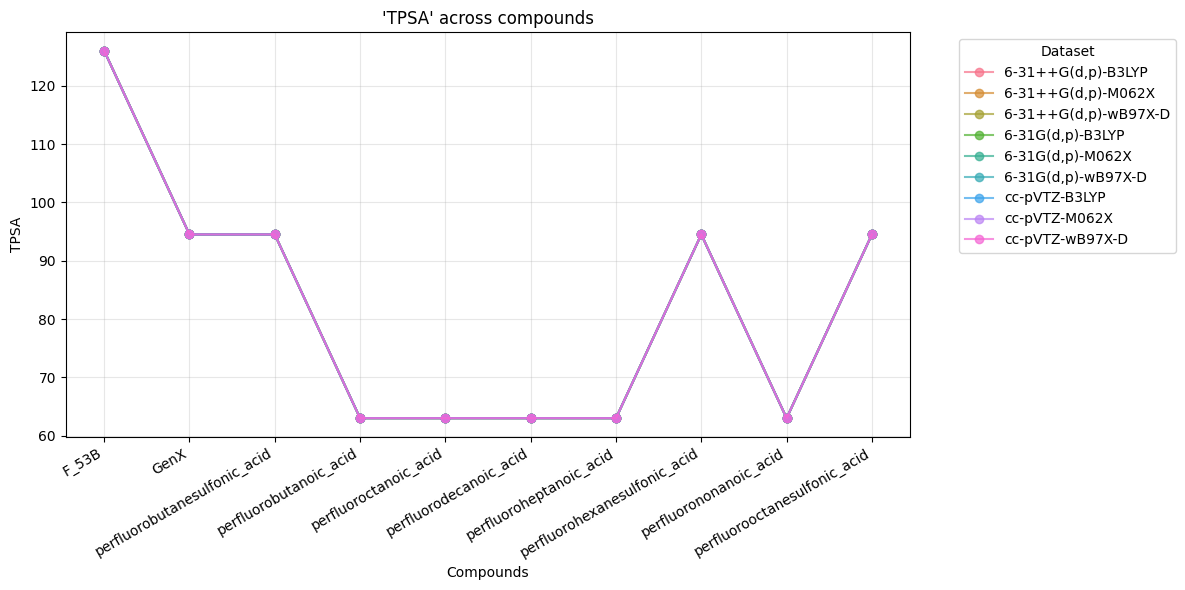
\includegraphics[width=\textwidth,height=\textheight,keepaspectratio]{Figures/plot_tpsa.png}
  \caption{Plot of topological polar surface area for each compound across all DFT methods.}
  \label{plot_tpsa}
\end{figure}

As shown in Figure. \ref{plot_sasa}, solvent-accessible surface area increases slightly when transitioning from 6-31G(d,p) to 6- 31++G(d,p), likely due to the inclusion of diffuse functions, and increases again when transitioning to cc-pVTZ. Perfluorobutanoic acid, for example, has an SASA of 164Å$^2$ at 6-31++G/B3LYP, 161Å$^2$ at 6-31G/B3LYP, and 163Å$^2$ at cc-pVTZ/B3LYP. Similar small variations are observed across all compounds. However, the general trend remains consistent: longer carbon chain correspond to proportionally larger surface area. Among the studied compounds, F53B has the largest SASA of all compounds (approximately 362Å$^2$ at 6-31++G/B3LYP and 360Å$^2$ at cc-pVTZ/B3LYP), while GenX has an intermediate SASA value (approximately 242Å$^2$ and 239Å$^2$, respectively). Sulfonic acids with carbon chain lengths comparable to those of carboxylic acids tend to exhibit slightly higher SASA values, likely due to the additional volume occupied by the sulfonate headgroup.

\begin{figure}[H]
  \centering
  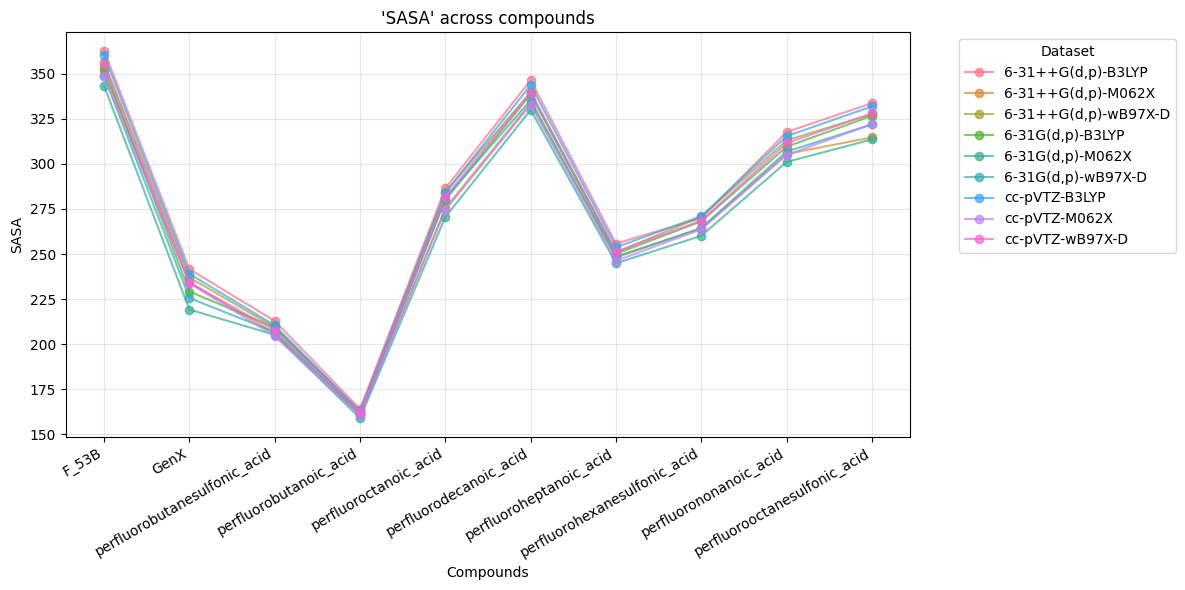
\includegraphics[width=\textwidth,height=\textheight,keepaspectratio]{Figures/plot_sasa.png}
  \caption{Plot of solvent accessible surface area (1.4Å water molecule probe) for each compound across all DFT methods.}
  \label{plot_sasa}
\end{figure}


\subsection{Frontier orbital energies and reactivity indices}

The energies of the highest occupied (HOMO) and lowest unoccupied (LUMO) molecular orbitals depend on the functional and basis set used (Figure \ref{plot_homo} and Figure \ref{plot_lumo}). However, clear trends emerge across different PFAS classes. Sulfonates and F53B consistently have more stable (i.e., lower) HOMO energies than carboxylates, indicating lower susceptibility to oxidation. Similarly, their LUMO energies are generally higher, indicating reduced electron affinity and a lower likelihood of undergoing reductive transformations.

\begin{figure}[H]
  \centering
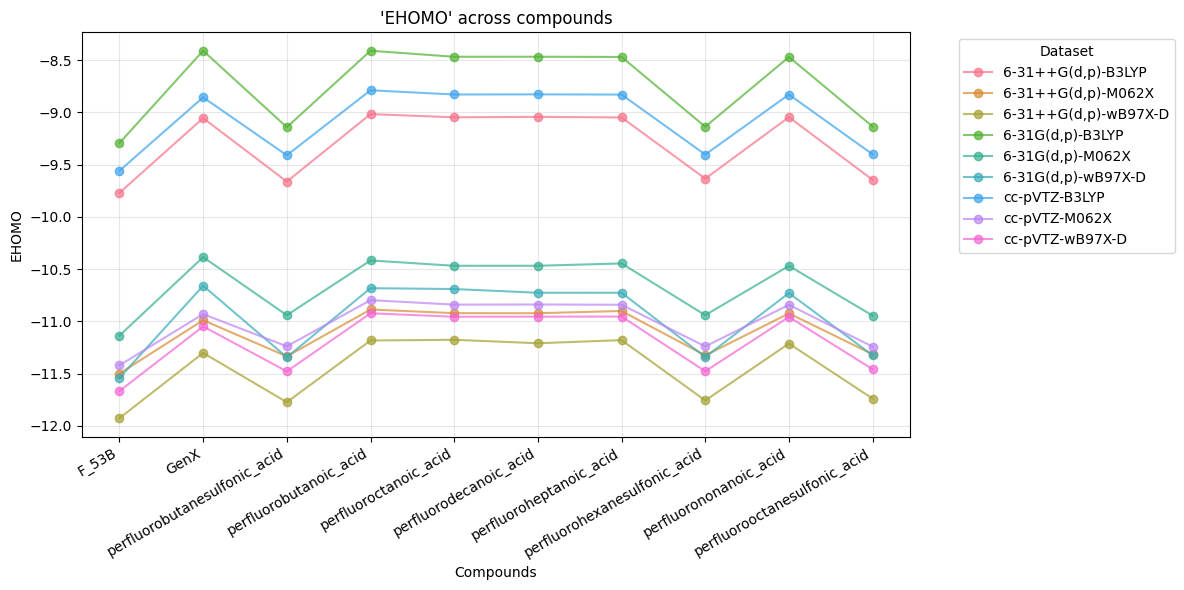
\includegraphics[width=\textwidth,height=\textheight,keepaspectratio]{Figures/plot_homo.png}
  \caption{Plot of HOMO energy for each compound across all DFT methods.}
  \label{plot_homo}
\end{figure}

\begin{figure}[H]
  \centering
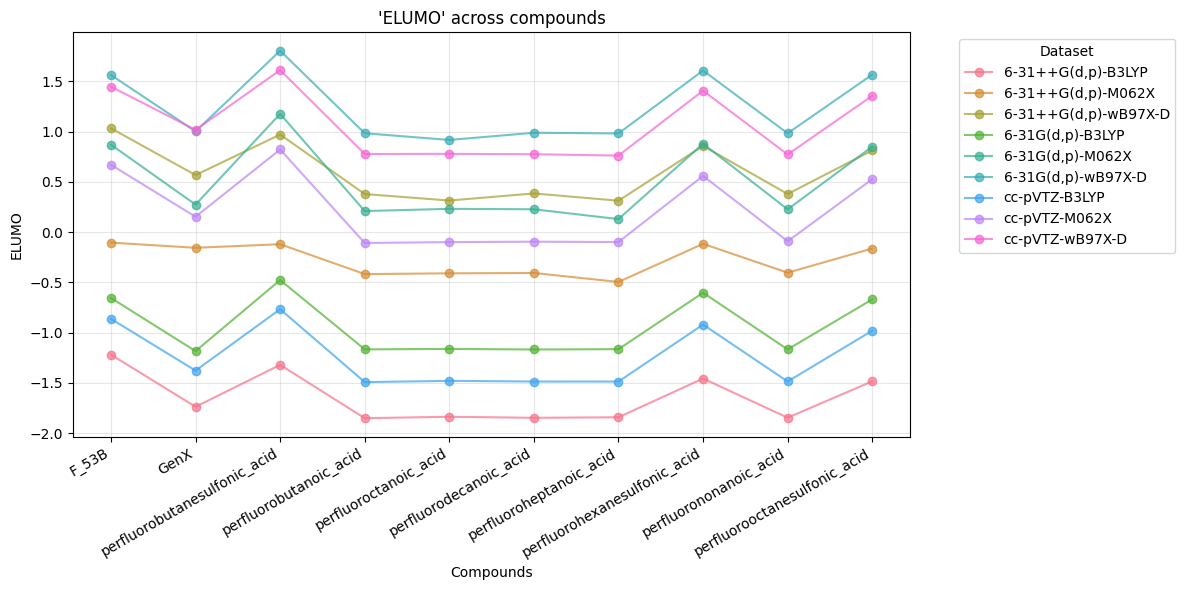
\includegraphics[width=\textwidth,height=\textheight,keepaspectratio]{Figures/plot_lumo.png}
  \caption{Plot of LUMO energy for each compound across all DFT methods.}
  \label{plot_lumo}
\end{figure}

The HOMO–LUMO gap, a key indicator of kinetic stability, is larger for sulfonates and F53B than for carboxylates (Figure \ref{plot_gap}). This suggests that these compounds are more chemically stable, consistent with their persistence in the environment and human body. GenX typically falls between these two groups, reflecting its hybrid structure.

\begin{figure}[H]
  \centering
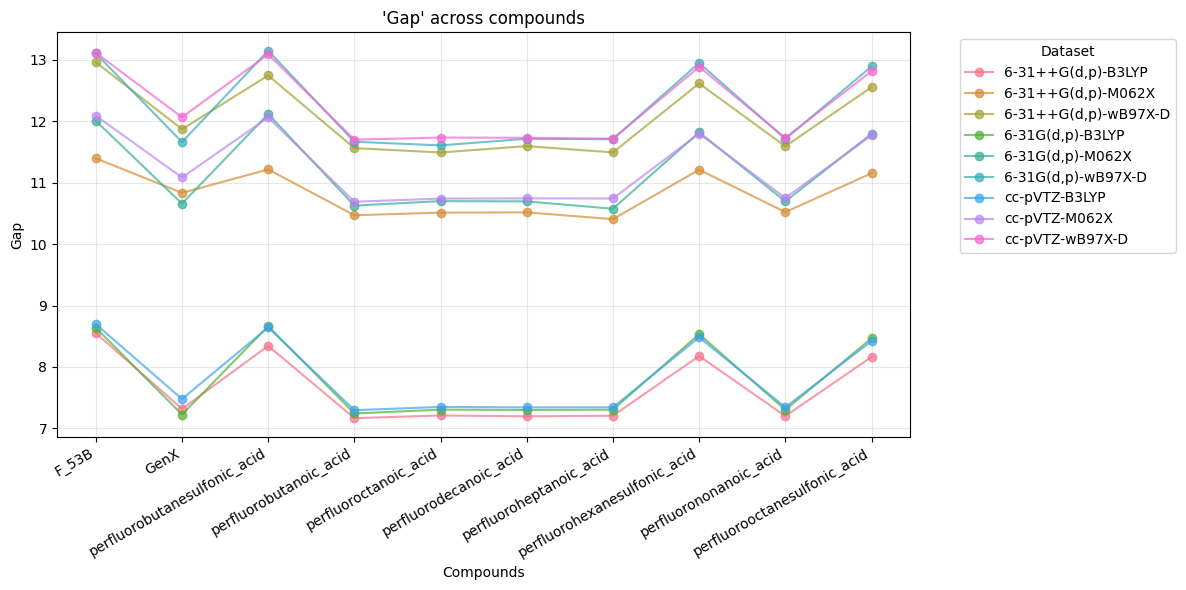
\includegraphics[width=\textwidth,height=\textheight,keepaspectratio]{Figures/plot_gap.png}
  \caption{Plot of HOMO-LUMO gap for each compound across all DFT methods.}
  \label{plot_gap}
\end{figure}

\begin{figure}[H]
  \centering
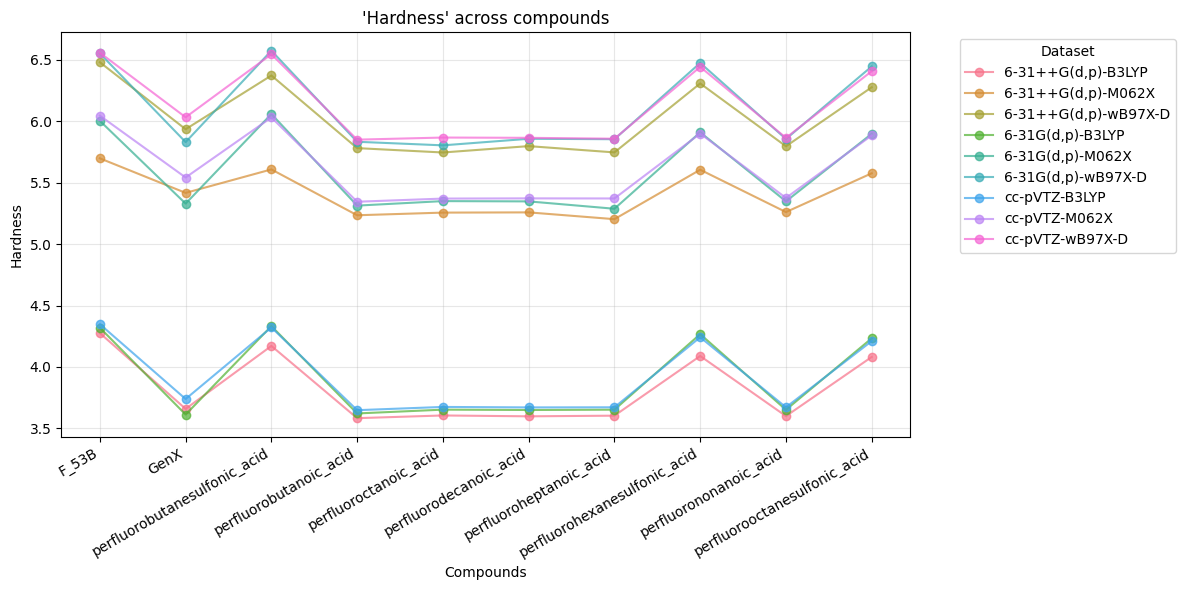
\includegraphics[width=\textwidth,height=\textheight,keepaspectratio]{Figures/plot_hardness.png}
  \caption{Plot of chemical hardness for each compound across all DFT methods.}
  \label{plot_hardness}
\end{figure}

\begin{figure}[H]
  \centering
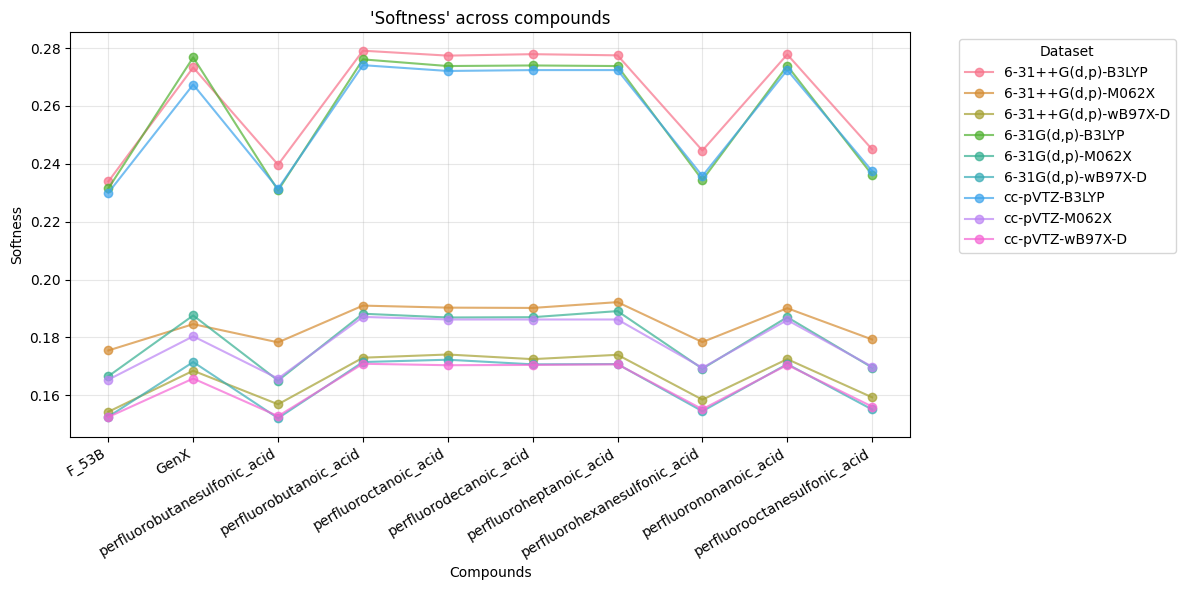
\includegraphics[width=\textwidth,height=\textheight,keepaspectratio]{Figures/plot_softness.png}
  \caption{Plot of chemical softness for each compound across all DFT methods.}
  \label{plot_softness}
\end{figure}

Similar to the HOMO–LUMO gap, chemical hardness ($\eta$) follows the similar pattern: sulfonates and F53B are harder, while carboxylates are softer and therefore more reactive (Figure \ref{plot_hardness}). This trend is important because softer, more reactive molecules tend to degrade more rapidly than harder molecules, which are generally more resistant to transformation.
Under B3LYP/6-31G(d,p), hardness for carboxylates lies around 3.6–3.7 eV, rising to ~4.1–4.3 eV for sulfonates or F53B when adding diffuse functions or moving to cc-pVTZ. Switching to M06-2X increases hardness by ~1.6–1.8 eV at each basis (e.g., perfluorobutanoic acid from ~3.58 to ~5.23 eV at 6-31++G(d,p)), and B97X-D further raises hardness by another ~0.5–0.8 eV (e.g., F53B hardness from ~4.28 eV under B3LYP/6-31++G(d,p) to ~6.48 eV under ωB97X-D/6-31++G(d,p)). Enlarging the basis from 6-31++G(d,p) to cc-pVTZ produces a modest additional increase (~0.1–0.3 eV) across functionals. Thus, both functional (more exact exchange) and larger basis sets systematically elevate hardness, reinforcing that method selection strongly influences predicted kinetic stability.  


Carboxylates, which feature lower hardness, show correspondingly higher softness, while sulfonates and F53B maintain lower softness across 3D-sensitive methods (Figure \ref{plot_softness}). Softness decreases (i.e., hardness increases) when progressing from \texttt{B3LYP} to \texttt{M06‑2X} and \texttt{$\omega$B97X‑D}, and when using larger basis sets such as \texttt{cc‑pVTZ}. For example, F53B softness drops from ~0.23 \texttt{(B3LYP/6‑31++G(d,p))} to ~0.15 \texttt{($\omega$B97X‑D/cc‑pVTZ)}, mirroring trends in gap and hardness.

\begin{figure}[H]
  \centering
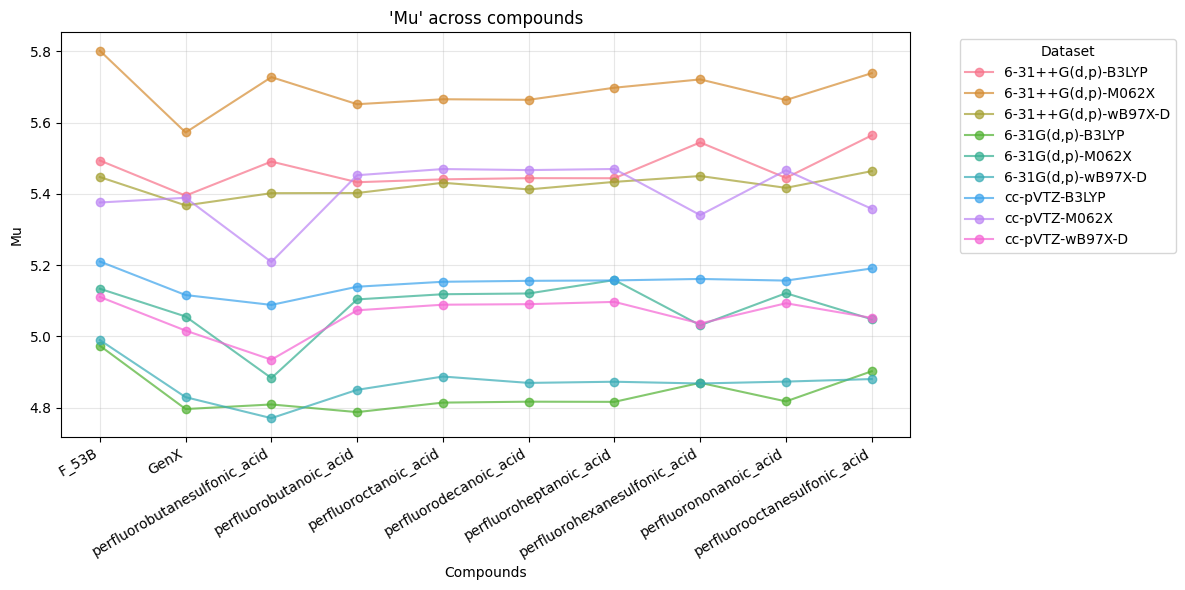
\includegraphics[width=\textwidth,height=\textheight,keepaspectratio]{Figures/plot_mu.png}
  \caption{Plot of chemical potential for each compound across all DFT methods.}
  \label{plot_mu}
\end{figure}

\begin{figure}[H]
  \centering
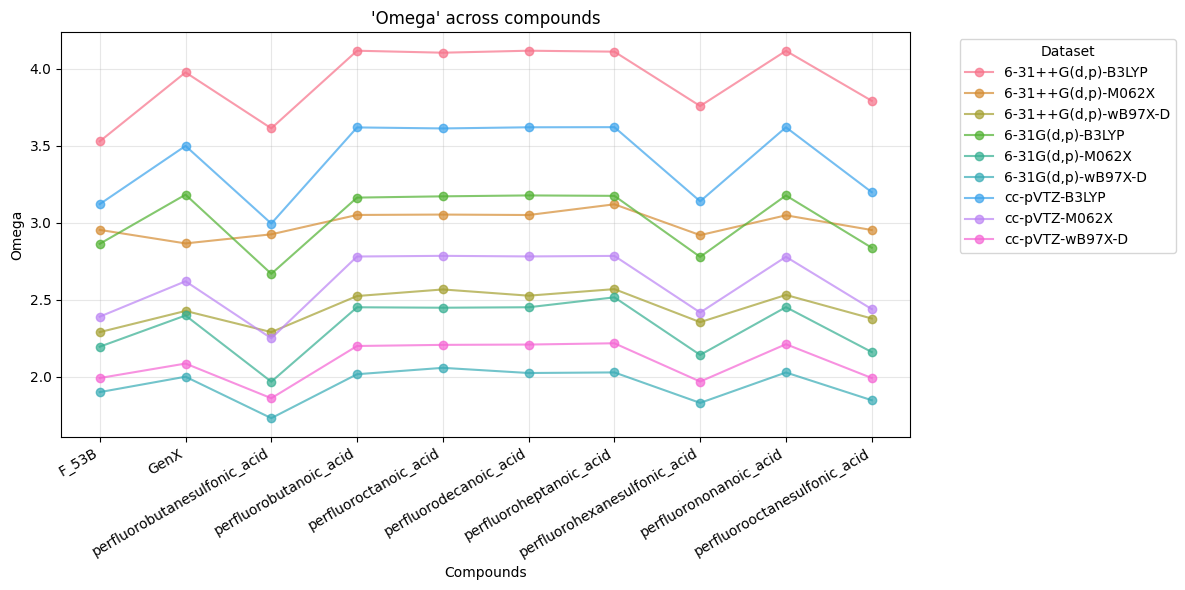
\includegraphics[width=\textwidth,height=\textheight,keepaspectratio]{Figures/plot_omega.png}
  \caption{Plot of electrophilicity index for each compound across all DFT methods.}
  \label{plot_omega}
\end{figure}

Although the chemical potential and electrophilicity index show smaller differences, they still support the same conclusion: sulfonates and F53B are somewhat less electrophilic, making them less likely to undergo reactions that could reduce their half-life (Figure \ref{plot_mu}). Chemical potential (μ) tends to be lower for B3LYP than for M06-2X, while ωB97X-D often yields values between or slightly below these, and enlarging the basis (from 6-31G(d,p) to 6-31++G(d,p) to cc-pVTZ) shifts μ modestly upward. Electrophilicity index (ω) shows a clearer downward trend when moving to higher-exact-exchange functionals and larger bases (Figure \ref{plot_omega}): B3LYP produces the highest ω, M06-2X lowers it, and ωB97X-D yields the lowest values; likewise, switching from 6-31++G(d,p) to cc-pVTZ further reduces ω. These shifts, though smaller than for gap or hardness, underscore that both functional and basis choice should meaningfully influence μ and ω magnitudes.


\subsection{Molecular dipole moments}

Molecular dipole moments are moderately sensitive to the choice of functional and the basis set (Figure \ref{plot_dipole}). At the B3LYP/6-31++G(d,p) level of theory, for example, the dipole moment of perfluorobutanoic acid is 3.93D, whereas the dipole moment of perfluoroctanoic acid is 3.18D. Perfluorobutanesulfonic acid and perfluorooctanesulfonic acid have dipole moments of 3.64D and 3.77D, respectively. GenX has a dipole of 3.30D, while F53B has a dipole of 4.64D. The inclusion of diffuse functions generally increases dipole moments by approximately 0.1–0.3D. Switching to the cc-pVTZ basis set, however, results in minor changes, typically within ±0.1D. Functionals that include a higher proportion of exact exchange, such as M06-2X and ωB97X-D, tend to yield slightly lower dipole moments than B3LYP (Figure \ref{plot_dipole}).

\begin{figure}[H]
  \centering
  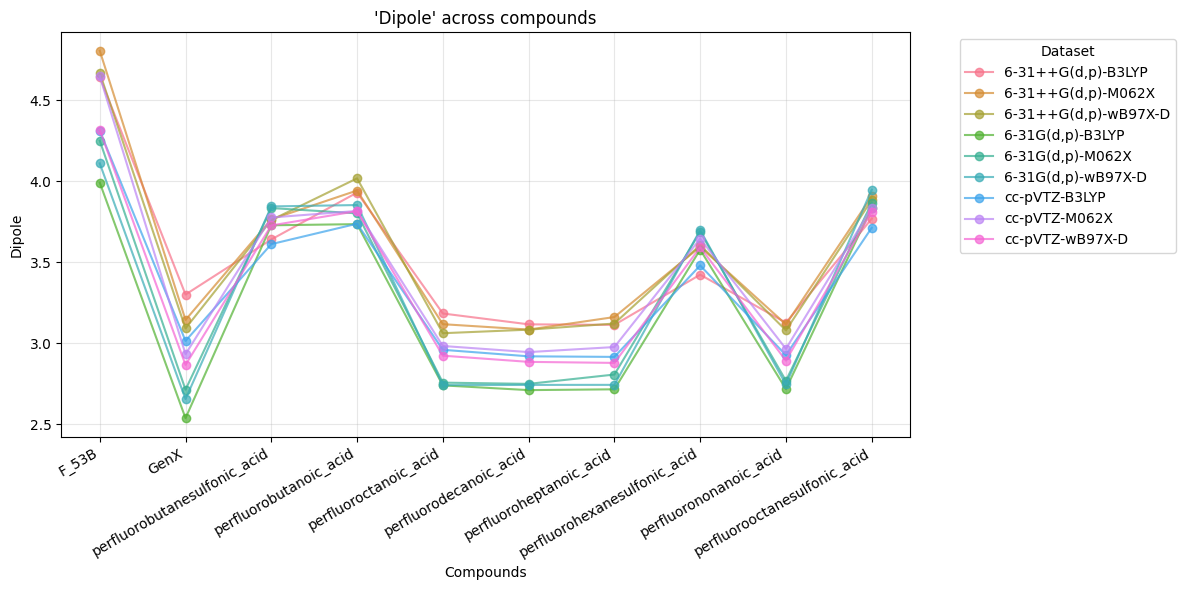
\includegraphics[width=\textwidth,height=\textheight,keepaspectratio]{Figures/plot_dipole.png}
  \caption{Plot of dipole moments for each compound across all DFT methods.}
  \label{plot_dipole}
\end{figure}


\section{Computational timing and trade-off analysis}

Calculation times increase significantly when using larger basis sets, more complex functionals, or when modeling larger molecules. For example, geometry optimization of perfluorobutanoic acid using B3LYP with the 6-31G(d,p) basis set takes approximately three minutes (Figure \ref{plot_time}). Adding diffuse functions (6-31++G(d,p)) increases computation time to around 19 minutes. Switching to the cc-pVTZ basis set increases computation time to approximately 116 minutes. For PFOA, the computation times are 27 minutes with B3LYP/6-31G(d,p), 270 minutes with B3LYP/6-31++G(d,p), and 1,291 minutes with B3LYP/cc-pVTZ. F53B the most computationally demanding molecule in this master’s project, requires 44 minutes at B3LYP/6-31G(d,p), 659 minutes at B3LYP/6-31++G(d,p), and 4980 minutes at B3LYP/cc-pVTZ.

Switching to the M06-2X functional generally increases computation times by a factor of approximately 1.2 to 1.5 for each basis set level. For instance, perfluorobutanoic acid requires five minutes at M06-2X/6-31G(d,p), 26 minutes at M06-2X/6-31++G(d,p), and 136 minutes at M06-2X/cc-pVTZ). The ωB97X-D functional is typically the most computationally intensive, increasing runtimes by an additional 20\% - 30\% compared to M06-2X for the same basis set (Figure \ref{plot_time}).

\begin{figure}[H]
  \centering
  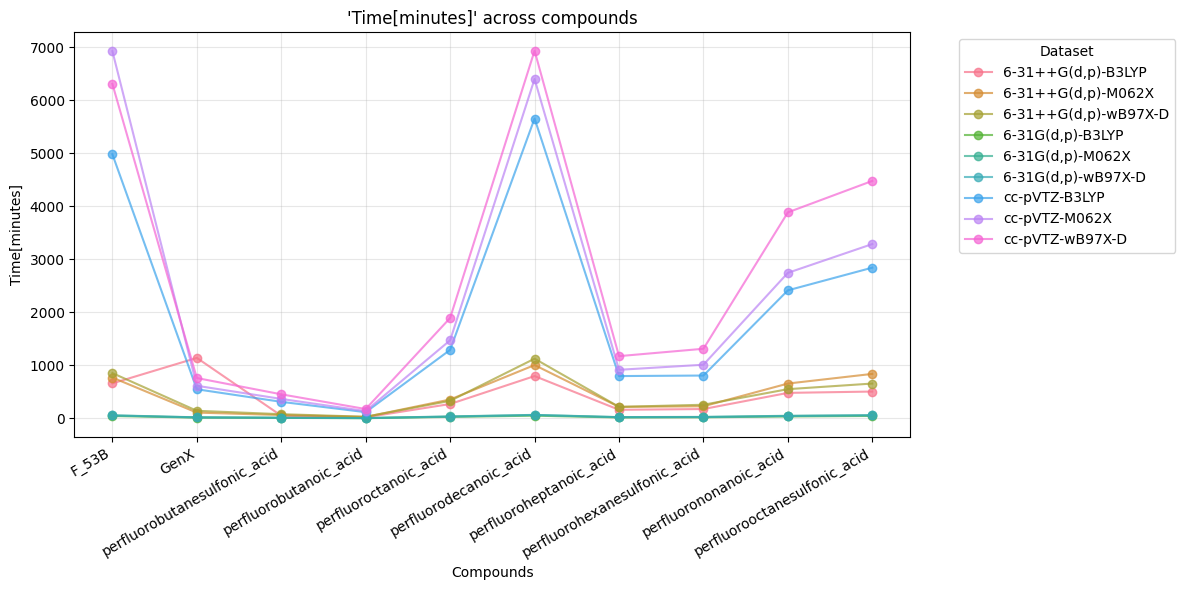
\includegraphics[width=\textwidth,height=\textheight,keepaspectratio]{Figures/plot_time.png}
  \caption{Plot of calculation time in minutes for each compound across all DFT methods.}
  \label{plot_time}
\end{figure}

Since calculation time scales approximately with the cube of the number of basis functions, longer perfluorocarbon chains, such as PFOA or PFDA, and more complex scaffolds, such as GenX or F53B, result in significantly longer runtimes at higher levels of theory. For routine descriptor generation, B3LYP combined with the 6-31G(d,p) basis set captures qualitative trends in chemical hardness, chemical softness, and orbital energies with minimal computational cost. However, accurate ELUMO values are needed for predicting reduction potentials or excited-state properties. In these cases, it is advisable to include diffuse functions (e.g., 6-31++G(d,p)) or, preferably, use a triple-ζ basis set, such as cc-pVTZ. Among the functionals tested, ωB97X-D generally provides the most reliable HOMO–LUMO gap values, albeit at the highest computational expense. M06-2X paired with 6-31++G(d,p) is a practical compromise that reproduces cc-pVTZ gap values within 0.1–0.2eV while requiring only about one-tenth of the computational time


\section{Group distinctions among PFAS, GenX, and F53B}

The perfluoroalkyl carboxylic acids (perfluorobutanoic acid, perfluorooctanoic acid, perfluorononanoic acid, perfluorodecanoic acid, and perfluoroheptanoic acid) exhibit a clear trend: as the fluorocarbon chain length increases, hydrophobicity also increases, while polar surface area and reactivity indices remain nearly constant. Regardless of the functional used, their EHOMO values cluster closely, and their electrophilicity indices fall within a narrow range.

In contrast, the perfluorosulfonic acids (perfluorobutanesulfonic acid, perfluorohexane- sulfonic acid, and perfluorooctanesulfonic acid) form a distinct group. They possess higher topological polar surface areas, slightly larger HOMO–LUMO gaps (and therefore greater chemical hardness), and correspondingly lower chemical softness compared to carboxylic acids of equivalent chain length. Their molecular dipole moments are typically 0.2–0.4D higher, and their chemical potentials are approximately 0.05–0.10eV more negative.

GenX acts as a bridges these two clusters. Its TPSA is comparable to that of sulfonates, yet its chemical hardness and softness more closely resemble those of medium-chain carboxylates. Under B3LYP/6-31++G(d,p), GenX exhibits ELUMO and EHOMO energies of –1.74eV and –9.05eV, respectively, resulting in a HOMO–LUMO gap of 7.32eV—nearly identical to that of PFOA (7.21eV). However, its dipole moment of 3.30D is slightly lower than that of PFOA (3.18D) and PFBS (3.64D). From a computational perspective, GenX requires significantly longer runtimes than PFAS molecules with comparable heavy-atom counts, due to its oxygenated and branched substituents. These increase the number of basis function and hinder convergence.

F53B is distinct from the PFCA and PFSA subgroups. It has the largest TPSA (126.0Å$^2$), the greatest dipole moment (up to 4.80D under M06-2X/6-31++G(d,p)), and the highest chemical hardness (up to 6.48eV under ωB97X-D/6-31++G(d,p)). These properties reflect its polyfunctional structure. However, F53B’s reactivity indices and polar surface area do not align cleanly with either group. The computational cost for F53B increases accordingly. At cc-pVTZ/ωB97XD, the runtime exceeds 6300 minutes (approximately 105 hours), highlighting that molecules of this complexity incur substantial computational overhead.


%----------------------------------------------------------------------------------------
\section{Influence of basis set and functional}

A two-way ANOVA was performed for each descriptor to evaluate the influence of the basis set, functional, and their interaction on computed molecular descriptors. Three levels of basis sets and three levels of functionals were used.

\clearpage
\subsection{Descriptors with no significant effects}

Neither the basis set, the functional, nor their interaction had a statistically significant effect on the following descriptors (all p > 0.05):

\begin{itemize}
    \item LogP (as value is not 3D-structure dependent)
    \item TPSA
    \item SASA
    \item HF Energy
    \item Dipole
\end{itemize}

These properties show minimal variation when different basis sets or functionals are used. This suggests that the choice of computational method does not significantly impact the results for these descriptors. Figures \ref{anova_logP}, \ref{anova_tpsa}, \ref{anova_sasa}, \ref{anova_hf} and \ref{anova_dipole} present nearly flat mean values across all combinations, confirming negligible method dependence.

\begin{figure}[H]
\centering
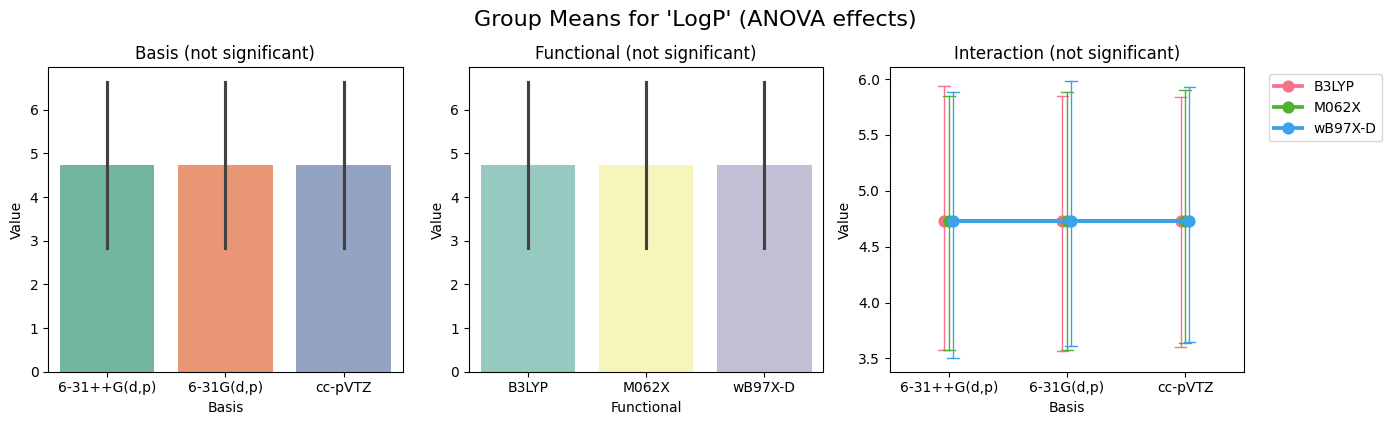
\includegraphics[width=\textwidth,height=\textheight,keepaspectratio]{Figures/anova_logP.png}
\caption{Group means for LogP. There were no significant effects observed for the basis set, the functional, or their combination.}
\label{anova_logP}
\end{figure}

\begin{figure}[H]
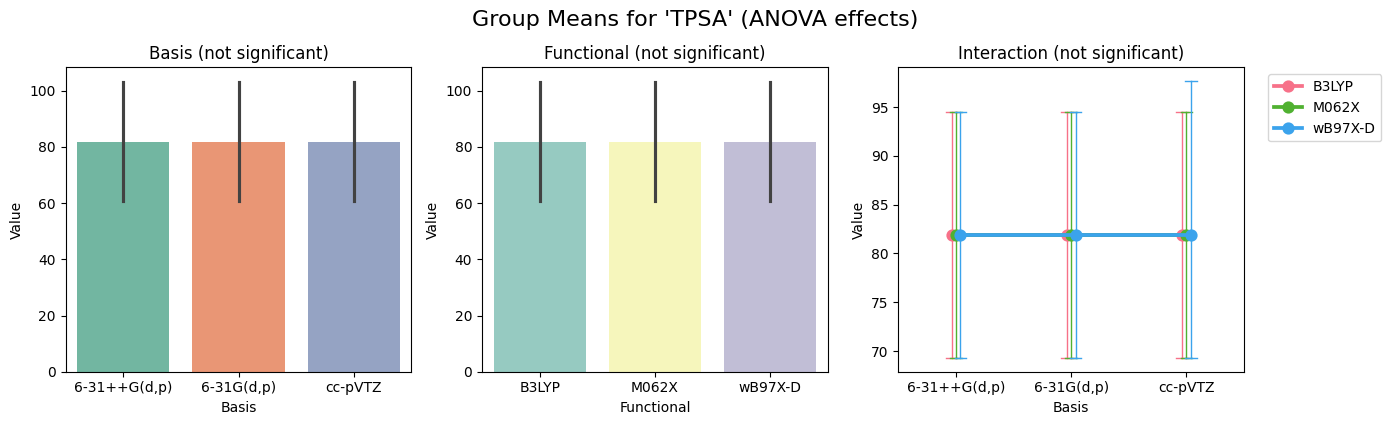
\includegraphics[width=\textwidth,height=\textheight,keepaspectratio]{Figures/anova_tpsa.png}
\caption{Group means for topological polar surface area. There were no significant effects observed for the basis set, the functional, or their combination.}
\label{anova_tpsa}
\end{figure}

\begin{figure}[H]
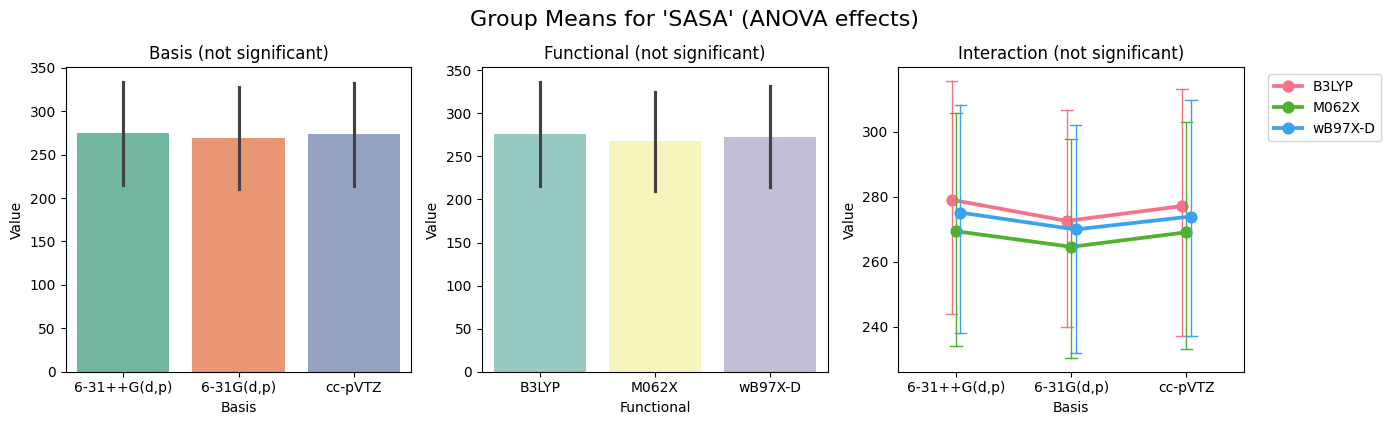
\includegraphics[width=\textwidth,height=\textheight,keepaspectratio]{Figures/anova_sasa.png}
\caption{Group means for solvent accessible surface area. There were no significant effects observed for the basis set, the functional or their combination.}
\label{anova_sasa}
\end{figure}

\begin{figure}[H]
\centering
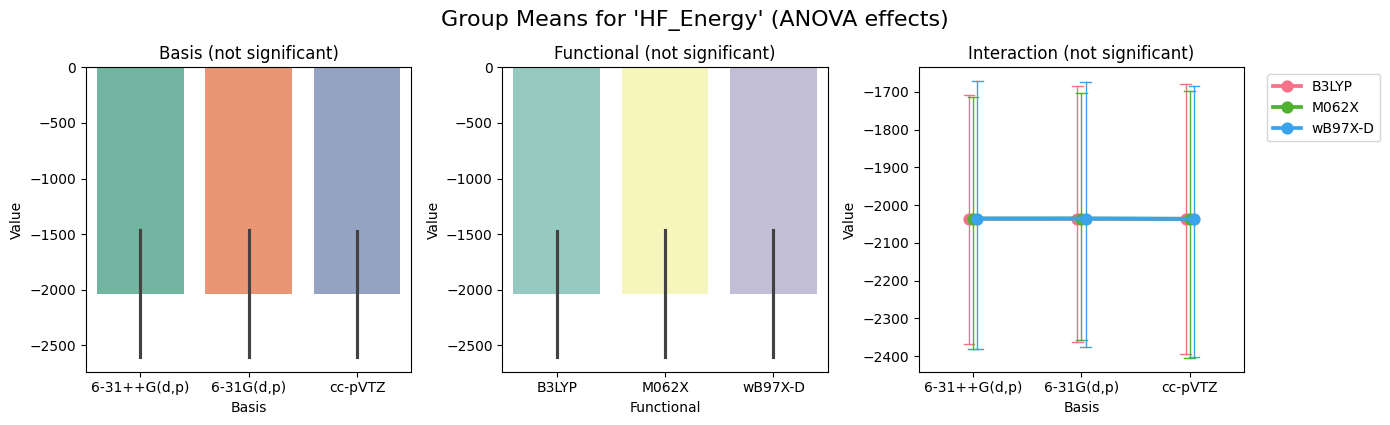
\includegraphics[width=\textwidth,height=\textheight,keepaspectratio]{Figures/anova_hf.png}
\caption{Group means for HF energy. There were no significant effects observed for the basis set, the functional or their combination.}
\label{anova_hf}
\end{figure}

\begin{figure}[H]
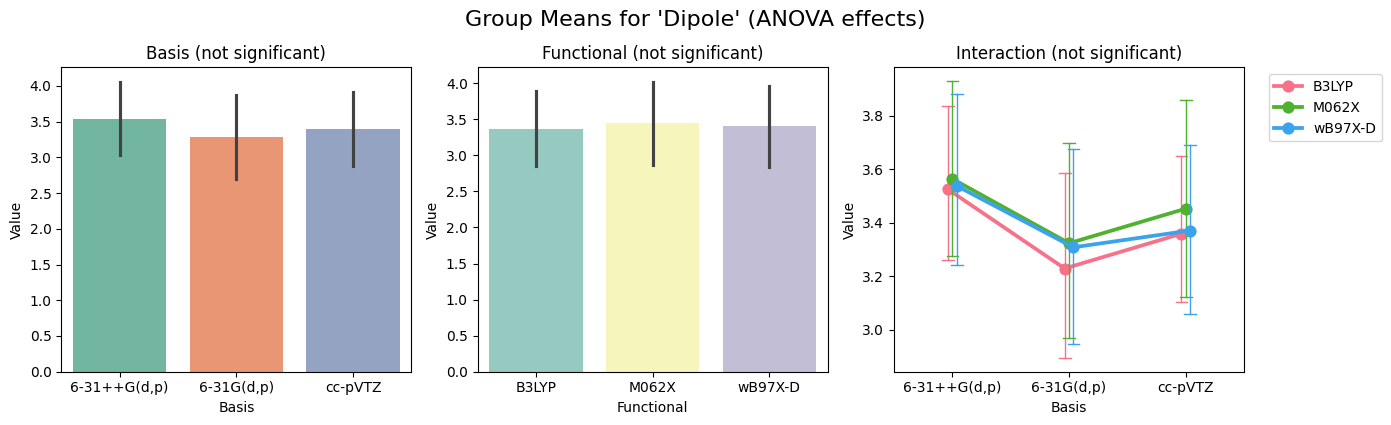
\includegraphics[width=\textwidth,height=\textheight,keepaspectratio]{Figures/anova_dipole.png}
\caption{Group means for total dipole moment. There were no significant effects observed for the basis set, the functional or their combination.}
\label{anova_dipole}
\end{figure}

\subsection{Descriptors with significant effects}
\subsection*{Descriptors with significant functional effects only}

The following descriptors and features had a statistically significant functional effect (p < 0.05), while the effects of the basis set and their interaction were not significant:

\begin{itemize}
    \item HOMO-LUMO Gap
    \item Chemical hardness
    \item Chemical softness
    \item Calculation time (not a descriptor)
\end{itemize}

\begin{figure}[H]
\centering
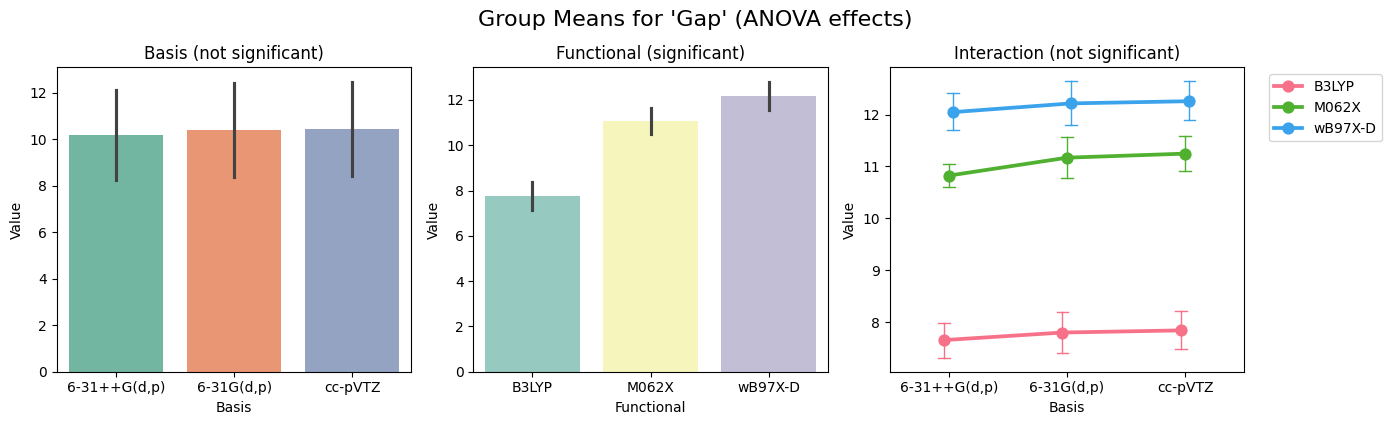
\includegraphics[width=\textwidth,height=\textheight,keepaspectratio]{Figures/anova_gap.png}
\caption{Group means for the HOMO-LUMO energy gap. The average energy gap grows with more complex functionals.}
\label{anova_gap}
\end{figure}

\begin{figure}[H]
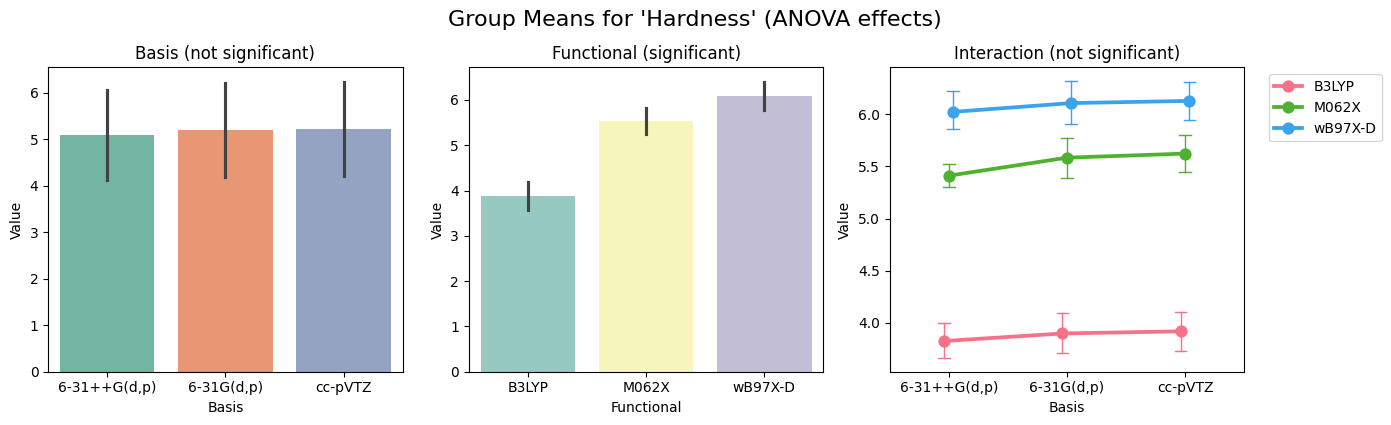
\includegraphics[width=\textwidth,height=\textheight,keepaspectratio]{Figures/anova_hardness.png}
\caption{Group means for the chemical hardness. The average chemical hardness increases with more complex functionals.}
\label{anova_hardness}
\end{figure}

\begin{figure}[H]
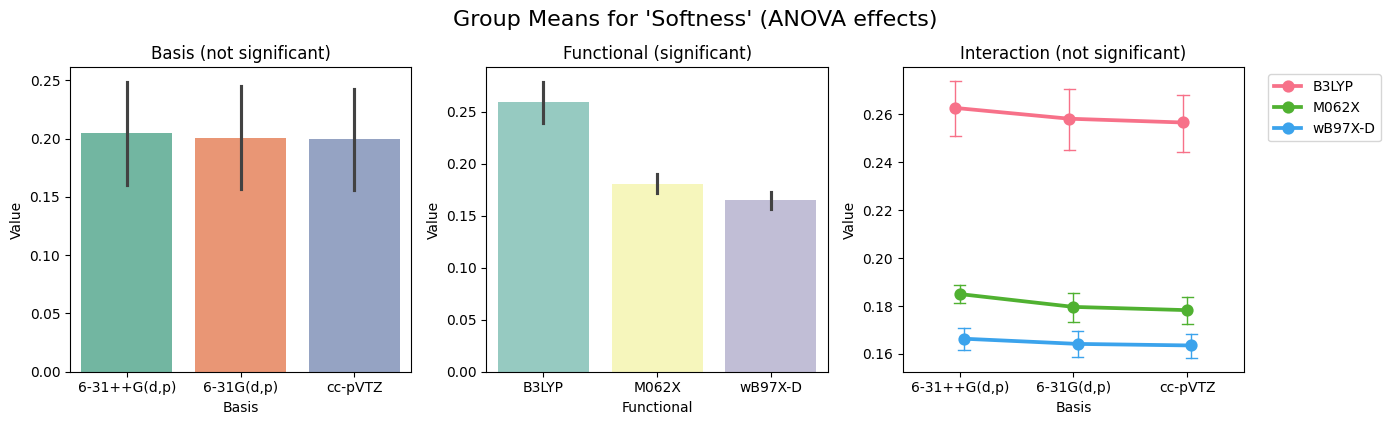
\includegraphics[width=\textwidth,height=\textheight,keepaspectratio]{Figures/anova_softness.png}
\caption{Group means for chemical softness. The average chemical hardness decreases with more complex functionals.}
\label{anova_softness}
\end{figure}

\begin{figure}[H]
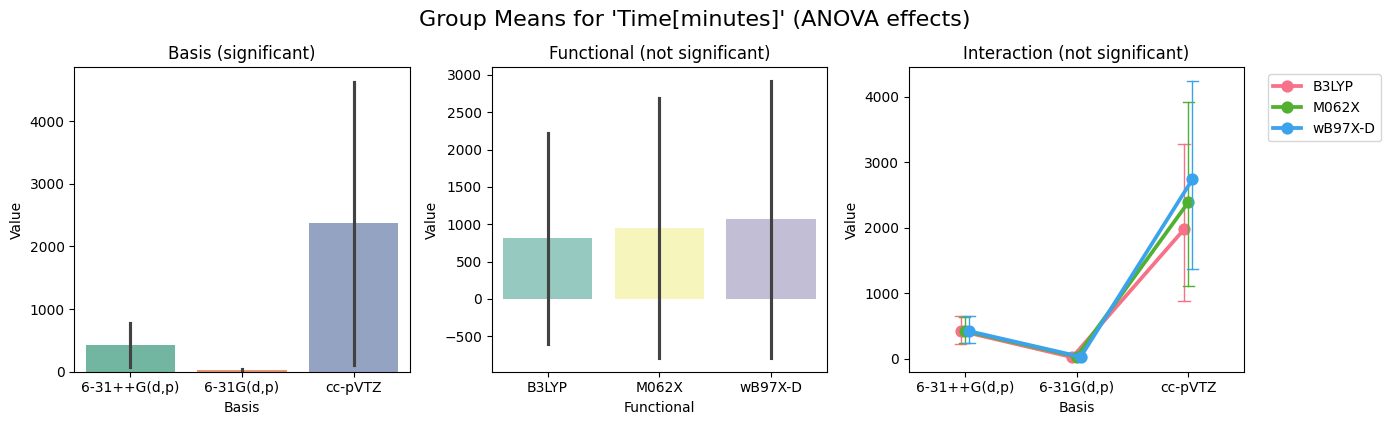
\includegraphics[width=\textwidth,height=\textheight,keepaspectratio]{Figures/anova_time.png}
\caption{Group means for time of calculation in minutes. We can see a big computational cost tradeoff with expanding basis set.}
\label{anova_time}
\end{figure}

\clearpage
The HOMO–LUMO gap varies notably across functionals (e.g., increasing from B3LYP to M06-2X to ωB97X-D), while basis-set changes produce only minor shifts (Figure \ref{anova_gap}). Likewise, chemical hardness and softness (Figures \ref{anova_hardness} and \ref{anova_softness}) follow similar trend: larger hardness and smaller softness values can be seen for functionals with more exact exchange. This confirms that frontier-derived descriptors are sensitive mainly to the exchange–correlation treatment, with negligible basis-set influence in this context.

\subsection*{Descriptors with significant basis and functional effects}

For EHOMO and ELUMO, both basis set and functional effects were highly significant (\(p \ll 0.05\)), but their interaction was not:

\begin{itemize}
    \item EHOMO: Basis (\(p = 1.69 \times 10^{-7}\)), Functional (\(p = 4.71 \times 10^{-44}\))
    \item ELUMO: Basis (\(p = 1.11 \times 10^{-12}\)), Functional (\(p = 2.16 \times 10^{-42}\))
\end{itemize}

\begin{figure}[H]
\centering
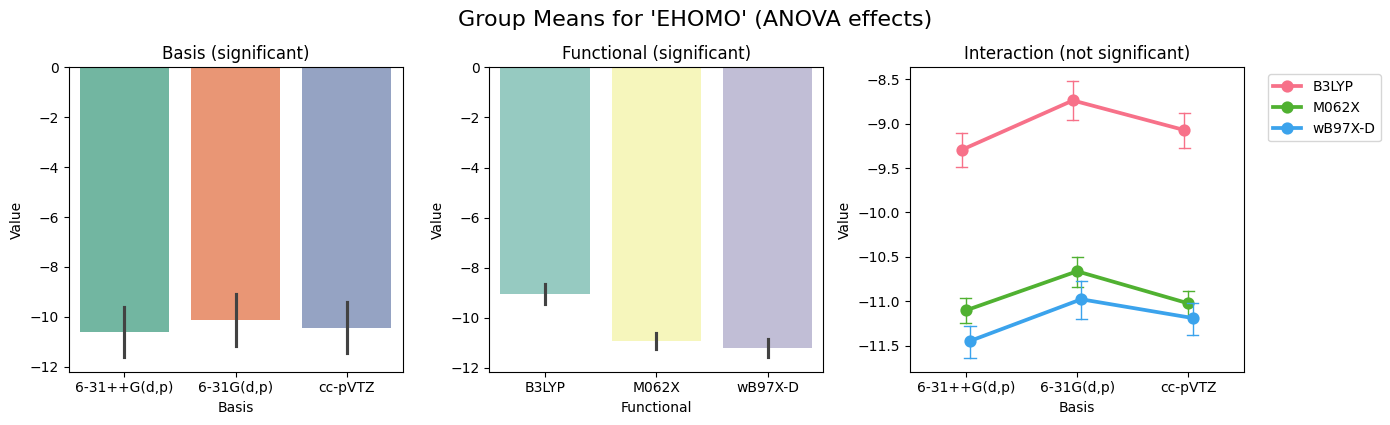
\includegraphics[width=\textwidth,height=\textheight,keepaspectratio]{Figures/anova_homo.png}
\caption{Group means for HOMO energy. Energy level seems to be changing across basis sets and growing with increasing functional complexity}
\label{anova_homo}
\end{figure}

\begin{figure}[H]
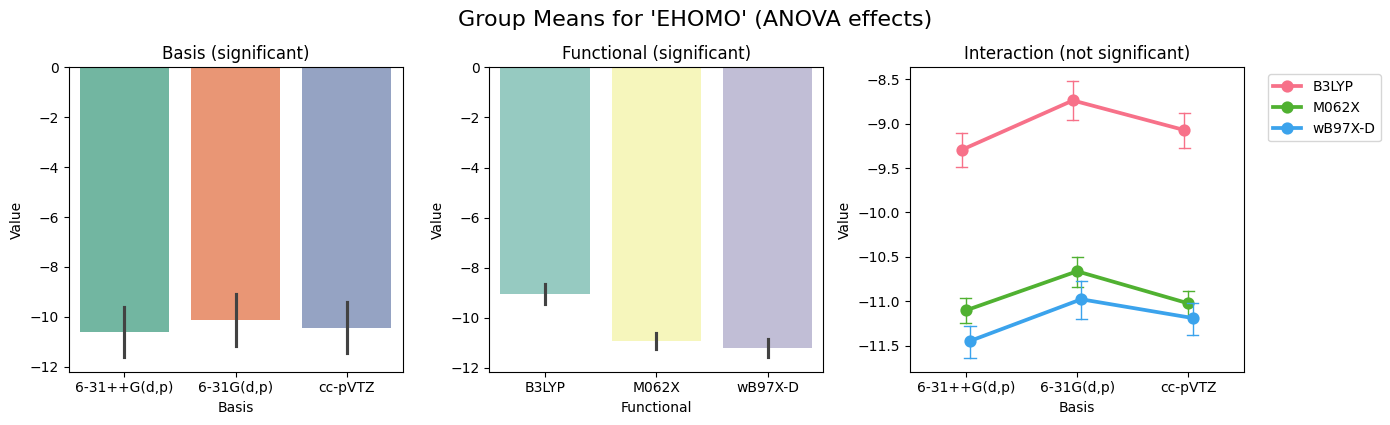
\includegraphics[width=\textwidth,height=\textheight,keepaspectratio]{Figures/anova_homo.png}
\caption{Group means for LUMO energy. Significant differences between different basis sets and functionals}
\label{anova_lumo}
\end{figure}

Both the basis set and functional independently influence the computed HOMO and LUMO energies. The lack of significant interaction indicates that the effect of one factor does not depend on the level of the other. EHOMO systematically deepens (more negative) when moving from B3LYP to M06-2X to ωB97X-D, and also shifts slightly downward with larger basis sets (Figures \ref{anova_homo} and \ref{anova_lumo}). Similarly, ELUMO energies shift upward or become more positive under functionals with more exact exchange and adjust modestly with basis size.


\subsection*{Descriptors with significant basis, functional, and interaction effects}

For Mu and Omega, all three effects were significant:

\begin{itemize}
    \item Mu: Basis (\(p = 1.45 \times 10^{-53}\)), Functional (\(p = 3.48 \times 10^{-31}\)), Interaction (\(p = 0.00506\))
    \item Omega: Basis (\(p = 2.96 \times 10^{-24}\)), Functional (\(p = 1.62 \times 10^{-42}\)), Interaction (\(p = 0.0155\))
\end{itemize}

\begin{figure}[H]
\centering
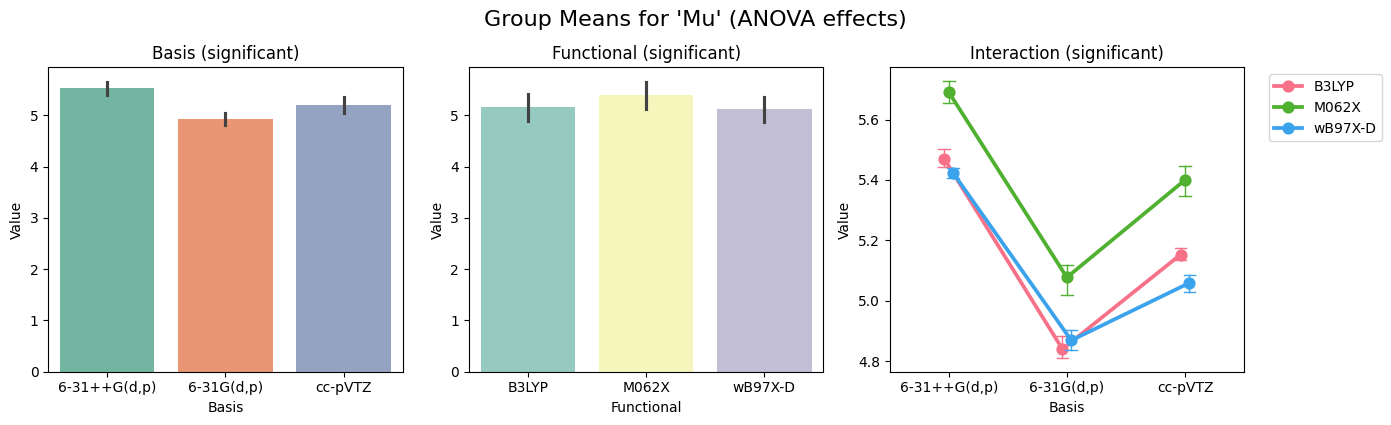
\includegraphics[width=\textwidth,height=\textheight,keepaspectratio]{Figures/anova_mu.png}
\caption{Group means for mu. Average value is smaller for 6-31G(d,p) basis set and larger for M062X functional}
\label{anova_mu}
\end{figure}

\begin{figure}[H]
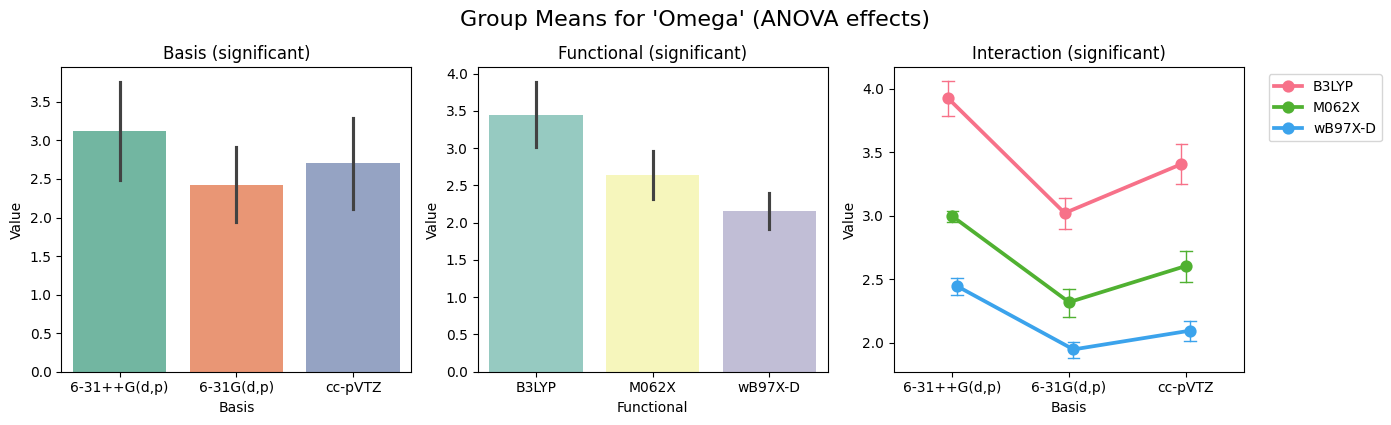
\includegraphics[width=\textwidth,height=\textheight,keepaspectratio]{Figures/anova_omega.png}
\caption{Group means for omega. The value is changing relative to the choice of basis set and dropping significantly with increasing functional complexity}
\label{anova_omega}
\end{figure}


 For chemical potential (Mu), mean values increase with larger basis sets but the magnitude of this increase differs by functional: e.g., M06-2X shows a larger rise from small to large basis than B3LYP or ωB97X-D (Figures \ref{anova_mu}). This interaction indicates that one cannot generalize a single basis effect across all functionals. For electrophilicity (Omega), values decrease going from B3LYP to M06-2X to ωB97X-D, and the basis-set enlargement moderates these shifts differently per functional Figure (\ref{anova_omega}). The visible trends underscore that both basis and functional choices jointly determine Mu and Omega, so a balanced mid-level combination (e.g., M06-2X/6-31++G(d,p)) may approximate higher-level results while controlling runtime.

Table~\ref{tab:anova-summary} summarizes the results of the two-way ANOVA performed for each descriptor and computational time, indicating which parameter(s) - basis set, functional, or their interaction - had a statistically significant effect.

\begin{table}[h!]
\centering
\caption{Summary of two-way ANOVA results for each descriptor. \textbf{Yes} = significant ($p < 0.05$), No = not significant.}
\begin{tabular}{lcccc}
\hline
\textbf{Descriptor} & \textbf{Basis} & \textbf{Functional} & \textbf{Interaction} & \textbf{Main Source of Variation} \\
\hline
LogP         & No  & No  & No  & None \\
TPSA         & No  & No  & No  & None \\
SASA         & No  & No  & No  & None \\
HF\_Energy   & No  & No  & No  & None \\
Dipole       & No  & No  & No  & None \\
Gap          & No  & \textbf{Yes} & No  & Functional \\
Hardness     & No  & \textbf{Yes} & No  & Functional \\
Softness     & No  & \textbf{Yes} & No  & Functional \\
EHOMO        & \textbf{Yes} & \textbf{Yes} & No  & Basis, Functional \\
ELUMO        & \textbf{Yes} & \textbf{Yes} & No  & Basis, Functional \\
Mu           & \textbf{Yes} & \textbf{Yes} & \textbf{Yes} & Basis, Functional, Interaction \\
Omega        & \textbf{Yes} & \textbf{Yes} & \textbf{Yes} & Basis, Functional, Interaction \\
Time         & \textbf{Yes} & No & No & Basis \\
\hline
\end{tabular}
\label{tab:anova-summary}
\end{table}


% --------------------------------------
% --------------------------------------
% --------------------------------------

\clearpage
\section{Machine learning results}
   

Using the descriptors (Sex, Species, LogP, SASA, Gap, HF energy) and dividing the nine PFAS compounds into a training set (6 compounds, as described above) and a test set (also described above), calculations were performed for nine basis sets with different functionals. Below are three tables corresponding to three machine learning methods – kNN, XGBoost, and Decision Tree (DT). The same descriptors were used in all calculations.

For the kNN algorithm (Table \ref{tab:my_table1}), the hyperparameter k was set to 3.
For XGBoost (Table \ref{tab:my_table2}), the parameters were: n estimators = 10, learning rate = 0.1, max depth = 3.
For the Decision Tree algorithm (Table \ref{tab:my_table3}), the parameters were: max depth = 3, min samples leaf = 10, min samples split = 3, random state = 42.

The results were compared in terms of performance using the calculated statistics: accuracy, precision, recall, and F1 score.


\begin{table}[H]
\centering
\caption{Results from all basis and functionals for kNN algorithm}
\begin{tabular}{|l |l |l |l |l |l |l |l |l|}\hline      
kNN& \multicolumn{2}{|c|}{Acuracy} & \multicolumn{2}{|c|}{Precision} & \multicolumn{2}{|c|}{Recall} & \multicolumn{2}{|c|}{F1} \\\hline
 & train & test & train & test & train & test & train & test \\\hline
6-31++G(d,p)-B3LYP & 0.947 & 0.818 & 0.953 & 0.709 & 0.947 & 0.818 & 0.947 & 0.75 \\\hline
6-31++G(d,p)-M062X & 0.947 & 0.818 & 0.953 & 0.709 & 0.947 & 0.818 & 0.947 & 0.75 \\\hline
6-31++G(d,p)-wB97X-D & 0.947 & 0.818 & 0.953 & 0.709 & 0.947 & 0.818 & 0.947 & 0.75 \\\hline
6-31G(d,p)-B3LYP & 0.947 & 0.818 & 0.953 & 0.709 & 0.947 & 0.818 & 0.947 & 0.75 \\\hline
6-31G(d,p)-M062X & 0.947 & 0.818 & 0.953 & 0.709 & 0.947 & 0.818 & 0.947 & 0.75 \\\hline
6-31G(d,p)-wB97X-D & 0.947 & 0.818 & 0.953 & 0.709 & 0.947 & 0.818 & 0.947 & 0.75 \\\hline
cc-pVTZ-B3LYP & 0.947 & 0.818 & 0.953 & 0.709 & 0.947 & 0.818 & 0.947 & 0.75 \\\hline
cc-pVTZ-M062X & 0.947 & 0.818 & 0.953 & 0.709 & 0.947 & 0.818 & 0.947 & 0.75 \\\hline
cc-pVTZ-wB97X-D & 0.947 & 0.818 & 0.953 & 0.709 & 0.947 & 0.818 & 0.947 & 0.75 \\ \hline

\end{tabular}
\label{tab:my_table1}
\end{table}


\begin{table}[H]
\centering
\caption{Results from all basis and functionals for XGBoost algorithm}
\begin{tabular}{|l |l |l |l |l |l |l |l |l|}\hline      
XGBoost& \multicolumn{2}{|c|}{Acuracy} & \multicolumn{2}{|c|}{Precision} & \multicolumn{2}{|c|}{Recall} & \multicolumn{2}{|c|}{F1} \\\hline
 & train & test & train & test & train & test & train & test \\\hline
6-31++G(d,p)-B3LYP & 0.929 & 0.727 & 0.942 & 0.609 & 0.929 & 0.727 & 0.929 & 0.660 \\\hline
6-31++G(d,p)-M062X & 0.929 & 0.727 & 0.942 & 0.609 & 0.929 & 0.727 & 0.929 & 0.660 \\\hline
6-31++G(d,p)-wB97X-D & 0.929 & 0.727 & 0.942 & 0.609 & 0.929 & 0.727 & 0.929 & 0.660 \\\hline
6-31G(d,p)-B3LYP & 0.929 & 0.727 & 0.942 & 0.609 & 0.929 & 0.727 & 0.929 & 0.660 \\\hline
6-31G(d,p)-M062X & 0.929 & 0.727 & 0.942 & 0.609 & 0.929 & 0.727 & 0.929 & 0.660 \\\hline
6-31G(d,p)-wB97X-D & 0.929 & 0.727 & 0.942 & 0.609 & 0.929 & 0.727 & 0.929 & 0.660 \\\hline
cc-pVTZ-B3LYP & 0.929 & 0.727 & 0.942 & 0.609 & 0.929 & 0.727 & 0.929 & 0.660 \\\hline
cc-pVTZ-M062X & 0.929 & 0.727 & 0.942 & 0.609 & 0.929 & 0.727 & 0.929 & 0.660 \\\hline
cc-pVTZ-wB97X-D & \textbf{0.894} & \textbf{0.909} & \textbf{0.899} & \textbf{0.927} & \textbf{0.894} & \textbf{0.909} & \textbf{0.895} & \textbf{0.905} \\ \hline

\end{tabular}
\label{tab:my_table2}
\end{table}



\begin{table}[H]
\centering
\caption{Results from all basis and functionals for DT algorithm}
\begin{tabular}{|l |l |l |l |l |l |l |l |l|}\hline      
DT & \multicolumn{2}{|c|}{Acuracy} & \multicolumn{2}{|c|}{Precision} & \multicolumn{2}{|c|}{Recall} & \multicolumn{2}{|c|}{F1} \\\hline
 & train & test & train & test & train & test & train & test \\\hline
6-31++G(d,p)-B3LYP & 0.807 & 0.727 & 0.848 & 0.609 & 0.807 & 0.727 & 0.809 & 0.660 \\\hline
6-31++G(d,p)-M062X & 0.807 & 0.727 & 0.848 & 0.609 & 0.807 & 0.727 & 0.809 & 0.660 \\\hline
6-31++G(d,p)-wB97X-D & 0.807 & 0.727 & 0.848 & 0.609 & 0.807 & 0.727 & 0.809 & 0.660 \\\hline
6-31G(d,p)-B3LYP & 0.807 & 0.727 & 0.848 & 0.609 & 0.807 & 0.727 & 0.809 & 0.660 \\\hline
6-31G(d,p)-M062X & 0.807 & 0.727 & 0.848 & 0.609 & 0.807 & 0.727 & 0.809 & 0.660 \\\hline
6-31G(d,p)-wB97X-D & 0.807 & 0.727 & 0.848 & 0.609 & 0.807 & 0.727 & 0.809 & 0.660 \\\hline
cc-pVTZ-B3LYP & 0.807 & 0.727 & 0.848 & 0.609 & 0.807 & 0.727 & 0.809 & 0.660 \\\hline
cc-pVTZ-M062X & 0.807 & 0.727 & 0.848 & 0.609 & 0.807 & 0.727 & 0.809 & 0.660 \\\hline
cc-pVTZ-wB97X-D & 0.736 & 0.727 & 0.772 & 0.609 & 0.736 & 0.727 & 0.737 & 0.660 \\ \hline

\end{tabular}

\label{tab:my_table3}
\end{table}

The results presented above apply to all tested databases and feature sets across three ma- chine learning algorithms — kNN, XGBoost, and DT. The cc-pVTZ-wB97X-D database in combination with the XGBoost algorithm achieved the best performance. These results are highlighted in bold in Table \ref{tab:my_table2}. For both the training and test sets, metrics such as accuracy, precision, recall, and F1 score are approximately 0.9, indicating very strong classification performance. Below is the confusion matrix  (Figure \ref{naj_conf_matrix}) for the aforementioned dataset. This represents the most accurate approach among those selected, although it is also the most time-consuming. In the training set, the XGBoost-based [Q]SPR model correctly classified:

\begin{itemize}
    \item 10 compounds in class 1
    \item 12 compounds in class 2
    \item 17 compounds in class 3
    \item 12 compounds in class 4
\end{itemize}
Six compounds were misclassified:
\begin{itemize}
    \item 1 compound from class 1 (perfluorooctanoic acid) was classified as class 3
    \item  3 compounds from class 2 (perfluorooctanoic acid and perfluorohexanesulfonic acid) were classified as class 3
    \item   2 compounds-rows from class 3 (perfluorobutanesulfonic acid for human male and female) were classified as class 2
\end{itemize}

This last type of misclassification is particularly concerning because class 3 corresponds to a half-life of less than 2 months, while class 2 corresponds to a half-life of less than one week. This means that the compound was mistakenly identified as less toxic than it actually is.

For the validation set, the algorithm correctly classified:
\begin{itemize}
    \item   4 compounds in class 1
    \item   4 compounds in class 2
    \item   8 compounds in class 3
    \item   4 compounds in class 4
\end{itemize}

Two compounds were misclassified:
\begin{itemize}
    \item from class 3 perfluorononanoic acid was classified as class 2
\end{itemize}

\begin{figure}[H]
    \centering
    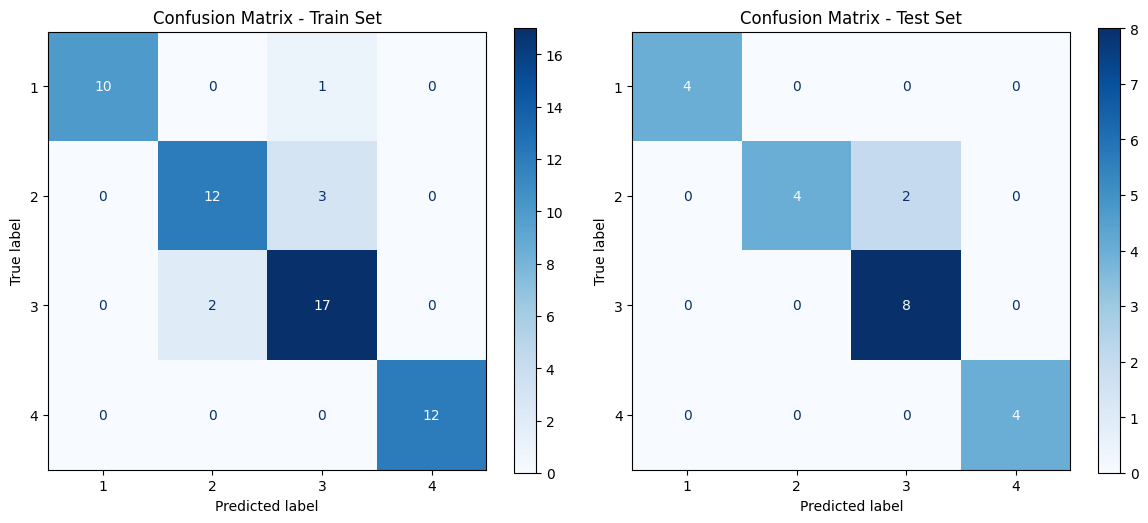
\includegraphics[width=\textwidth,height=\textheight,keepaspectratio]{Figures/naj_conf_matrix.png}
    \caption{Confusion matrix of the best-performing XGBoost-based [Q]SPR model for classifying PFAS into categories based on their half-life}
    \label{naj_conf_matrix}
\end{figure}



For better visualization of the data and results, the table below presents the data along with descriptors, the name of the compound, the class half lifetime, and the prediction from the selected model — XGB for $\omega$B97X-D/cc-pVTZ.


\begin{table}[H]
\caption{Dataset used during model development. Colored rows indicate incorrect prediction of half-life class.}
\resizebox{\textwidth}{!}{%
\begin{tabular}{|l|l|l|l|l|l|l|l|l|l|}
\hline
\textbf{Name} & \textbf{Species} & \textbf{Sex} & \textbf{LogP} & \textbf{SASA} & \textbf{Gap} & \textbf{HF\_Energy} & \textbf{T/V} & \textbf{Class half   lifetime} & \multicolumn{1}{c|}{\textbf{Predictions}} \\ \hline
GenX & Human & Male & 3.266 & 176.5496 & 12.0639 & -1553.3455 & T & 2 & 2 \\ \hline
GenX & Rat & Male & 3.266 & 176.5496 & 12.0639 & -1553.3455 & T & 2 & 2 \\ \hline
GenX & Monkey & Female & 3.266 & 176.5496 & 12.0639 & -1553.3455 & T & 2 & 2 \\ \hline
GenX & Rat & Male & 3.266 & 176.5496 & 12.0639 & -1553.3455 & T & 2 & 2 \\ \hline
GenX & Monkey & Male & 3.266 & 176.5496 & 12.0639 & -1553.3455 & T & 2 & 2 \\ \hline
GenX & Rat & Female & 3.266 & 176.5496 & 12.0639 & -1553.3455 & T & 2 & 2 \\ \hline
GenX & Human & Female & 3.266 & 176.5496 & 12.0639 & -1553.3455 & T & 2 & 2 \\ \hline
GenX & Rat & Female & 3.266 & 176.5496 & 12.0639 & -1553.3455 & T & 2 & 2 \\ \hline
GenX & Mouse & Female & 3.266 & 176.5496 & 12.0639 & -1553.3455 & T & 2 & 2 \\ \hline
GenX & Mouse & Male & 3.266 & 176.5496 & 12.0639 & -1553.3455 & T & 2 & 2 \\ \hline
Perfluoroheptanoic   acid & Human & Male & 5.0318 & 193.5779 & 11.7148 & -1715.9077 & T & 4 & 4 \\ \hline
Perfluoroheptanoic   acid & Rat & Male & 5.0318 & 193.5779 & 11.7148 & -1715.9077 & T & 1 & 1 \\ \hline
Perfluoroheptanoic   acid & Rat & Female & 5.0318 & 193.5779 & 11.7148 & -1715.9077 & T & 1 & 1 \\ \hline
Perfluoroheptanoic   acid & Rat & Female & 5.0318 & 193.5779 & 11.7148 & -1715.9077 & T & 1 & 1 \\ \hline
Perfluoroheptanoic   acid & Human & Female & 5.0318 & 193.5779 & 11.7148 & -1715.9077 & T & 4 & 4 \\ \hline
Perfluoroheptanoic   acid & Rat & Male & 5.0318 & 193.5779 & 11.7148 & -1715.9077 & T & 1 & 1 \\ \hline
Perfluorooctanoic   acid & Monkey & Male & 5.9729 & 219.0702 & 11.7338 & -1953.7174 & T & 3 & 3 \\ \hline
Perfluorooctanoic   acid & Rat & Male & 5.9729 & 219.0702 & 11.7338 & -1953.7174 & T & 3 & 3 \\ \hline
Perfluorooctanoic   acid & Human & Male & 5.9729 & 219.0702 & 11.7338 & -1953.7174 & T & 4 & 4 \\ \hline
Perfluorooctanoic   acid & Mouse & Male & 5.9729 & 219.0702 & 11.7338 & -1953.7174 & T & 3 & 3 \\ \hline
\rowcolor[HTML]{DAE9F8} 
Perfluorooctanoic   acid & Rat & Female & 5.9729 & 219.0702 & 11.7338 & -1953.7174 & T & 2 & 3 \\ \hline
Perfluorooctanoic   acid & Rat & Male & 5.9729 & 219.0702 & 11.7338 & -1953.7174 & T & 3 & 3 \\ \hline
Perfluorooctanoic   acid & Monkey & Male & 5.9729 & 219.0702 & 11.7338 & -1953.7174 & T & 3 & 3 \\ \hline
Perfluorooctanoic   acid & Mouse & Female & 5.9729 & 219.0702 & 11.7338 & -1953.7174 & T & 3 & 3 \\ \hline
\rowcolor[HTML]{DAE9F8} 
Perfluorooctanoic   acid & Rat & Female & 5.9729 & 219.0702 & 11.7338 & -1953.7174 & T & 1 & 3 \\ \hline
Perfluorooctanoic   acid & Human & Female & 5.9729 & 219.0702 & 11.7338 & -1953.7174 & T & 4 & 4 \\ \hline
Perfluorooctanoic   acid & Monkey & Female & 5.9729 & 219.0702 & 11.7338 & -1953.7174 & T & 3 & 3 \\ \hline
Perfluorooctanesulfonic   acid & Mouse & Female & 5.566 & 255.4005 & 12.8136 & -2626.7966 & T & 3 & 3 \\ \hline
Perfluorooctanesulfonic   acid & Human & Female & 5.566 & 255.4005 & 12.8136 & -2626.7966 & T & 4 & 4 \\ \hline
Perfluorooctanesulfonic   acid & Monkey & Female & 5.566 & 255.4005 & 12.8136 & -2626.7966 & T & 4 & 4 \\ \hline
Perfluorooctanesulfonic   acid & Human & Male & 5.566 & 255.4005 & 12.8136 & -2626.7966 & T & 4 & 4 \\ \hline
Perfluorooctanesulfonic   acid & Rat & Female & 5.566 & 255.4005 & 12.8136 & -2626.7966 & T & 3 & 3 \\ \hline
Perfluorooctanesulfonic   acid & Mouse & Male & 5.566 & 255.4005 & 12.8136 & -2626.7966 & T & 3 & 3 \\ \hline
Perfluorooctanesulfonic   acid & Rat & Male & 5.566 & 255.4005 & 12.8136 & -2626.7966 & T & 3 & 3 \\ \hline
Perfluorooctanesulfonic   acid & Monkey & Male & 5.566 & 255.4005 & 12.8136 & -2626.7966 & T & 4 & 4 \\ \hline
Perfluorooctanesulfonic   acid & Rat & Male & 5.566 & 255.4005 & 12.8136 & -2626.7966 & T & 3 & 3 \\ \hline
Perfluorooctanesulfonic   acid & Rat & Female & 5.566 & 255.4005 & 12.8136 & -2626.7966 & T & 3 & 3 \\ \hline
Perfluorobutanesulfonic   acid & Rat & Female & 1.8016 & 153.4312 & 13.0892 & -1675.5 & T & 1 & 1 \\ \hline
Perfluorobutanesulfonic   acid & Monkey & Male & 1.8016 & 153.4312 & 13.0892 & -1675.5 & T & 2 & 2 \\ \hline
Perfluorobutanesulfonic   acid & Mouse & Female & 1.8016 & 153.4312 & 13.0892 & -1675.5 & T & 1 & 1 \\ \hline
Perfluorobutanesulfonic   acid & Mouse & Male & 1.8016 & 153.4312 & 13.0892 & -1675.5 & T & 1 & 1 \\ \hline
\rowcolor[HTML]{DAE9F8} 
Perfluorobutanesulfonic   acid & Human & Male & 1.8016 & 153.4312 & 13.0892 & -1675.5 & T & 3 & 2 \\ \hline
Perfluorobutanesulfonic   acid & Rat & Male & 1.8016 & 153.4312 & 13.0892 & -1675.5 & T & 1 & 1 \\ \hline
Perfluorobutanesulfonic   acid & Monkey & Female & 1.8016 & 153.4312 & 13.0892 & -1675.5 & T & 2 & 2 \\ \hline
Perfluorobutanesulfonic   acid & Rat & Male & 1.8016 & 153.4312 & 13.0892 & -1675.5 & T & 1 & 1 \\ \hline
\rowcolor[HTML]{DAE9F8} 
Perfluorobutanesulfonic   acid & Human & Female & 1.8016 & 153.4312 & 13.0892 & -1675.5 & T & 3 & 2 \\ \hline
Perfluorobutanesulfonic   acid & Rat & Female & 1.8016 & 153.4312 & 13.0892 & -1675.5 & T & 1 & 1 \\ \hline
Perfluorohexanesulfonic   acid & Mouse & Female & 3.6838 & 204.4159 & 12.8838 & -2151.1801 & T & 3 & 3 \\ \hline
Perfluorohexanesulfonic   acid & Rat & Male & 3.6838 & 204.4159 & 12.8838 & -2151.1801 & T & 3 & 3 \\ \hline
Perfluorohexanesulfonic   acid & Human & Male & 3.6838 & 204.4159 & 12.8838 & -2151.1801 & T & 4 & 4 \\ \hline
Perfluorohexanesulfonic   acid & Human & Female & 3.6838 & 204.4159 & 12.8838 & -2151.1801 & T & 4 & 4 \\ \hline
Perfluorohexanesulfonic   acid & Monkey & Male & 3.6838 & 204.4159 & 12.8838 & -2151.1801 & T & 4 & 4 \\ \hline
Perfluorohexanesulfonic   acid & Rat & Male & 3.6838 & 204.4159 & 12.8838 & -2151.1801 & T & 3 & 3 \\ \hline
Perfluorohexanesulfonic   acid & Mouse & Male & 3.6838 & 204.4159 & 12.8838 & -2151.1801 & T & 3 & 3 \\ \hline
\rowcolor[HTML]{DAE9F8} 
Perfluorohexanesulfonic   acid & Rat & Female & 3.6838 & 204.4159 & 12.8838 & -2151.1801 & T & 2 & 3 \\ \hline
\rowcolor[HTML]{DAE9F8} 
Perfluorohexanesulfonic   acid & Rat & Female & 3.6838 & 204.4159 & 12.8838 & -2151.1801 & T & 2 & 3 \\ \hline
Perfluorohexanesulfonic   acid & Monkey & Female & 3.6838 & 204.4159 & 12.8838 & -2151.1801 & T & 4 & 4 \\ \hline

\end{tabular}%
}
\end{table}


\begin{table}[H]
\resizebox{\textwidth}{!}{%
\begin{tabular}{|l|l|l|l|l|l|l|l|l|l|}
\hline
\textbf{Name} & \textbf{Species} & \textbf{Sex} & \textbf{LogP} & \textbf{SASA} & \textbf{Gap} & \textbf{HF\_Energy} & \textbf{T/V} & \textbf{Class half   lifetime} & \multicolumn{1}{c|}{\textbf{Predictions}} \\ \hline
Perfluorononanoic   acid & Rat & Male & 6.914 & 244.5625 & 11.7295 & -2191.5274 & V & 3 & 3 \\ \hline
Perfluorononanoic   acid & Human & Male & 6.914 & 244.5625 & 11.7295 & -2191.5274 & V & 4 & 4 \\ \hline
Perfluorononanoic   acid & Human & Female & 6.914 & 244.5625 & 11.7295 & -2191.5274 & V & 4 & 4 \\ \hline
Perfluorononanoic   acid & Rat & Male & 6.914 & 244.5625 & 11.7295 & -2191.5274 & V & 3 & 3 \\ \hline
Perfluorononanoic   acid & Mouse & Female & 6.914 & 244.5625 & 11.7295 & -2191.5274 & V & 3 & 3 \\ \hline
\rowcolor[HTML]{DAE9F8} 
Perfluorononanoic   acid & Rat & Female & 6.914 & 244.5625 & 11.7295 & -2191.5274 & V & 2 & 3 \\ \hline
\rowcolor[HTML]{DAE9F8} 
Perfluorononanoic   acid & Rat & Female & 6.914 & 244.5625 & 11.7295 & -2191.5274 & V & 2 & 3 \\ \hline
Perfluorononanoic   acid & Mouse & Male & 6.914 & 244.5625 & 11.7295 & -2191.5274 & V & 3 & 3 \\ \hline
Perfluorobutanoic   acid & Human & Female & 2.2085 & 117.1009 & 11.6995 & -1002.4773 & V & 2 & 2 \\ \hline
Perfluorobutanoic   acid & Monkey & Male & 2.2085 & 117.1009 & 11.6995 & -1002.4773 & V & 2 & 2 \\ \hline
Perfluorobutanoic   acid & Monkey & Female & 2.2085 & 117.1009 & 11.6995 & -1002.4773 & V & 2 & 2 \\ \hline
Perfluorobutanoic   acid & Human & Male & 2.2085 & 117.1009 & 11.6995 & -1002.4773 & V & 2 & 2 \\ \hline
Perfluorobutanoic   acid & Rat & Male & 2.2085 & 117.1009 & 11.6995 & -1002.4773 & V & 1 & 1 \\ \hline
Perfluorobutanoic   acid & Mouse & Male & 2.2085 & 117.1009 & 11.6995 & -1002.4773 & V & 1 & 1 \\ \hline
Perfluorobutanoic   acid & Mouse & Female & 2.2085 & 117.1009 & 11.6995 & -1002.4773 & V & 1 & 1 \\ \hline
Perfluorobutanoic   acid & Rat & Female & 2.2085 & 117.1009 & 11.6995 & -1002.4773 & V & 1 & 1 \\ \hline
Perfluorodecanoic   acid & Human & Male & 7.8551 & 270.0549 & 11.7292 & -2429.3374 & V & 4 & 4 \\ \hline
Perfluorodecanoic   acid & Rat & Female & 7.8551 & 270.0549 & 11.7292 & -2429.3374 & V & 3 & 3 \\ \hline
Perfluorodecanoic   acid & Rat & Male & 7.8551 & 270.0549 & 11.7292 & -2429.3374 & V & 3 & 3 \\ \hline
Perfluorodecanoic   acid & Rat & Male & 7.8551 & 270.0549 & 11.7292 & -2429.3374 & V & 3 & 3 \\ \hline
Perfluorodecanoic   acid & Rat & Female & 7.8551 & 270.0549 & 11.7292 & -2429.3374 & V & 3 & 3 \\ \hline
Perfluorodecanoic   acid & Human & Female & 7.8551 & 270.0549 & 11.7292 & -2429.3374 & V & 4 & 4 \\ \hline
\end{tabular}%
}
\end{table}

Of particular note is the fact that the average computation time required to perform geometry optimization and calculate descriptors for a single compound was 39 hours, as shown in (Figure \ref{times}). Due to the significant time and computational costs involved, as well as the fact that the best-performing descriptor calculation method described above did not substantially improve classification results compared to other considered methods, the question of balancing accuracy with computational efficiency arises. It is important to remember that \textit{in silico} models, including the [Q]SPR model developed in this master’s thesis, are approximations of experimental results.
     

\begin{figure}[H]
    \centering
    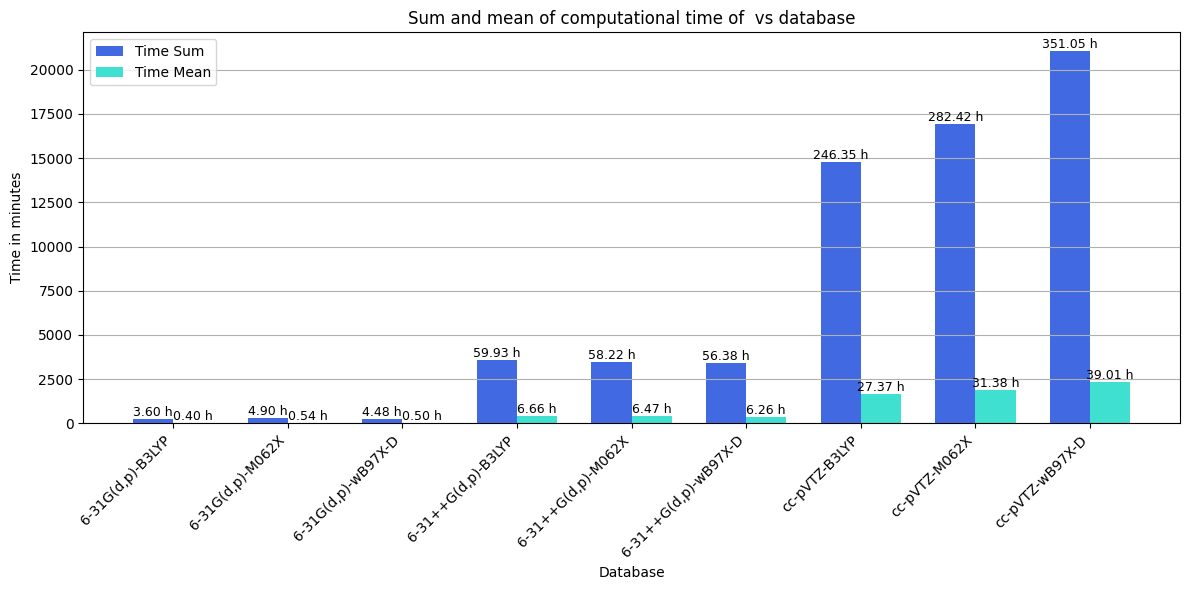
\includegraphics[width=\textwidth,height=\textheight,keepaspectratio]{Figures/times_sum_mean.png}
    \caption{Bar plot, of the sum and mean of the computational time for the considered DFT methods (combining various functionals with different basis sets).}
    \label{times}
\end{figure}

It can be seen that for many basis sets and functionals, the results are very similar. For example, in the case of the kNN algorithm, the evaluation statistics are the same for several combinations.
When comparing a model that has lower performance based on the calculated statistics but much shorter computation time, this observation becomes even clearer. For example, for the 6-31++G(d,p) basis set with the M06-2X functional, the confusion matrix for the XGBoost algorithm is shown in the figure \ref{conf_M062}.


From the results table above, it can be observed that the model is slightly overfitted, as the accuracy for the training data is 0.92, while for the test data it drops to 0.72.
The confusion matrix shows good prediction performance for the training set, with only 3 compounds misclassified.
However, for the test set, as before, 2 compounds were incorrectly assigned to class 3 instead of class 2. Additionally, in this case, no compound was correctly classified into class 1.

\begin{figure}[H]
    \centering
    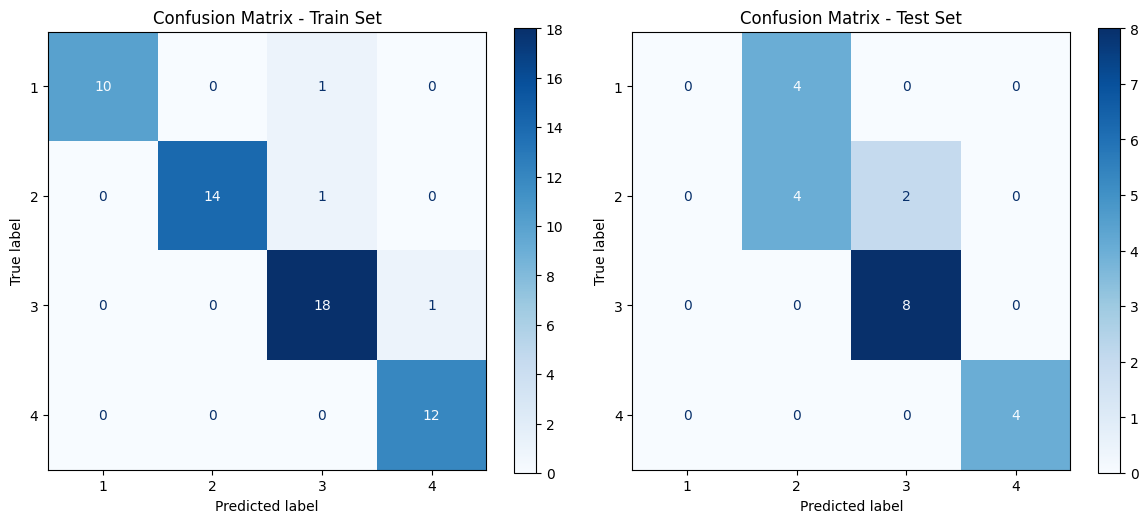
\includegraphics[width=\textwidth,height=\textheight,keepaspectratio]{Figures/conf_matrix_m062.png}
    \caption{Confusion matrix for XGBoost classifier trained and tested for M06-2X/6-31++G(d,p)}
    \label{conf_M062}
\end{figure}


The XGBoost model's feature importance analysis, based on gain values, highlights the HOMO-LUMO gap as the most influential feature, contributing 27\% to the model's predictive power. This is followed by SASA at 23\%, and HF energy at 17\%, indicating the dominant role of electronic and structural molecular properties. Species identity and logP also play substantial roles, contributing 16\% and 15\%, respectively. Notably, Sex shows minimal influence at only 3\%, suggesting that the molecular features are the primary drivers of the model's performance, while demographic factors like sex have limited predictive value in this context \ref{fig:feature_importance}.

\begin{figure}[H]
    \centering
    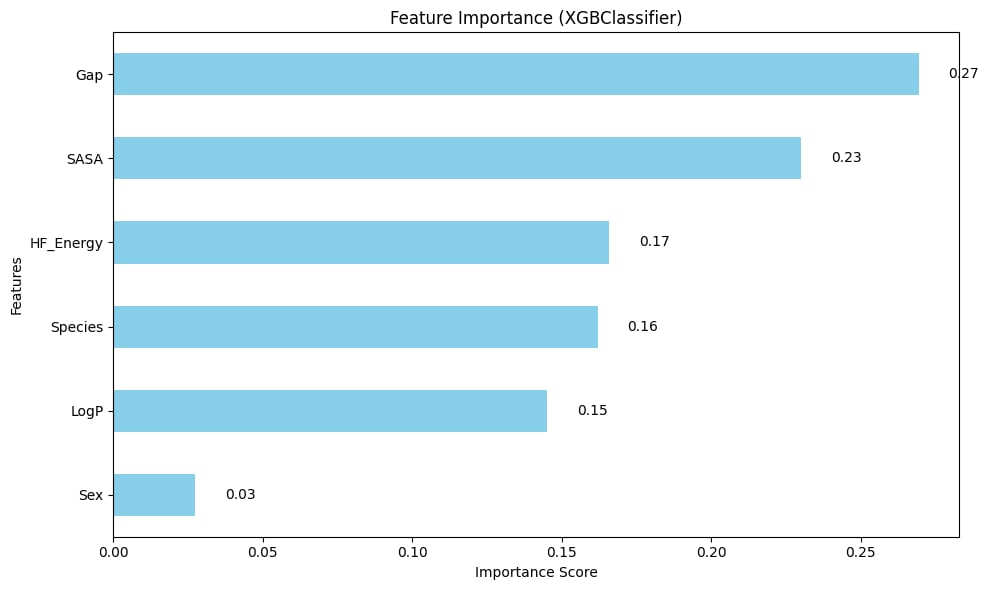
\includegraphics[width=\textwidth,height=\textheight,keepaspectratio]{Figures/feataure_imporatnce.jpg}
    \caption{Feature importance plot for XGB algorithm for the most accurate model.}
    \label{fig:feature_importance}
\end{figure}
% #wykres dodamy w wynikach

% -------------------------------------------
% -------------------------------------------
% -------------------------------------------
% -------------------------------------------
% -------------------------------------------

\chapter{Discussion}

In this section, we interpret the findings from both the DFT-derived descriptor analysis and the machine learning experiments. Specifically, we examine how methodological choices, particularly the basis set, functional, influence descriptor values and their reliability in classifying PFAS persistence. We also explore the trade-offs between computational cost and descriptor accuracy. Next, we evaluate the performance of these descriptors in PFAS half-life category classification models. Finally, we compare different ML algorithms and descriptor sets and reflect on the earlier outlined research hypotheses and objectives.

\subsection{DFT-derived descriptors: influence of functional and basis set}

A central aim of this master’s thesis was to understand how the choice of exchange–correlation functional and basis set affect the computed molecular descriptors that may correlate with PFAS persistence (Objectives 1 and 2). The results of two-way ANOVA revealed distinct patterns. Descriptors such as LogP, TPSA, SASA, HF energy, and dipole moment were largely unaffected by the basis set or functional choice (all \(p>0.05\)). These results suggest that a modest level of theor (e.g., \texttt{B3LYP}/\texttt{6-31G(d,p)}) ) is sufficient to obtain stable values for these properties. From a practical standpoint, these descriptors can be efficiently computed with minimal sensitivity to methodological variation, enabling the allocation of computational resources toward more sensitive quantities.

In contrast, the energies of frontier orbitals (i.e., EHOMO and ELUMO) showed significant dependence on both the basis set and the functional. This suggests that predicted orbital levels and derived descriptors, such as the HOMO-LUMO gap, and chemical hardness, are sensitive to the level of theory. Specifically, the energies of the HOMO and LUMO energies became more negative with increasing basis set size and with functionals containing a higher proportion of exact exchange. Since the HOMO–LUMO gap is fundamental to secondary descriptors such as chemical hardness (\(\eta\)), chemical softness, chemical potential (\(\mu\)), and electrophilicity (\(\omega\)), these properties also varied significantly with methodological choices. Notably, the HOMO–LUMO gap, chemical hardness and chemical softness were significantly affected by the functional alone, while \(\mu\) and \(\omega\) were influenced by the basis set, functional, and their interaction. These results suggest that, although HOMO–LUMO gap-related descriptors are primarily sensitive to the exchange–correlation treatment, the basis set and functional play critical roles in determining chemical potential and electrophilicity. 

From a chemical perspective, descriptors related to frontier orbitals are key to understanding PFAS stability. Larger HOMO–LUMO gaps and higher chemical hardness are generally associated with greater resistance to oxidative or reductive degradation and therefore longer half-lives. However, their sensitivity to the computational method implies that selecting an appropriate level of theory is essential to balancing accuracy and computational feasibility. For example, \texttt{B3LYP}/\texttt{6-31G(d,p)} can capture qualitative trends, such as the relative ordering among PFAS classes, but it tends to underestimate HOMO–LUMO gap values compared to higher-level methods, such as (e.g., \texttt{\(\omega\)B97X-D}/\texttt{cc-pVTZ}). While the latter provides more robust quantitative results, it comes at a significantly higher computational cost. 

The significant interaction effects observed for \(\mu\) and \(\omega\) imply that the impact of the functional on these descriptors depends on the basis set size and \textit{vice versa}. In practice, using a mid-level basis set (e.g., \texttt{6-31++G(d,p)}) with a balanced functional (e.g., \texttt{M06-2X}) yields descriptor values that closely approximate those of high-level methods while maintaining manageable runtimes. When comparing HOMO–LUMO gaps computed at \texttt{M06‑2X/6‑31++G(d,p)} to those obtained at the higher-level \texttt{M06‑2X/cc‑pVTZ} level, deviations of approximately 0.2–0.3 eV are observed for perfluoroalkyl carboxylates, while sulfonates and bulkier PFAS compounds exhibit larger deviations ranging from $\sim$0.5 to 0.9 eV. Notably, despite these differences, no degradation in predictive performance was observed in machine learning models trained on either descriptor set, indicating the adequacy of the more affordable \texttt{M06‑2X/6‑31++G(d,p)} method for model construction in this context. Thus, for large-scale descriptor generation (Objective 3), this level of theory appears to offer a practical compromise—capturing essential electronic structure features relevant to PFAS persistence while operating at approximately one-tenth the computational cost of \texttt{cc‑pVTZ}.

Overall, these findings support research hypotheses H2 and H3 that descriptor quality and model performance vary depending on the chosen DFT method, and that more expensive methods do not necessarily offer the best trade-off. The invariance of certain descriptors suggests that they can be reliably computed at low cost, while more method-sensitive descriptors require careful methodological selection.

\subsection{Descriptor trends and PFAS persistence insights}

Beyond methodological sensitivity, the absolute and relative values of molecular descriptors reveal the distinct chemical characteristics of PFAS classes:

\paragraph{HOMO–LUMO gap, chemical hardness, chemical softness.} 
Sulfonates and bulky compounds, such as F53B, consistently exhibit larger HOMO–LUMO gaps and greater chemical hardness than carboxylates with similar chain lengths. This aligns with their known environmental and biological persistence \cite{F53B_worse} \cite{F53B_worse_2}. GenX occupies an intermediate position, reflecting its hybrid structural nature. This trend highlights the importance of frontier orbital-derived descriptors in modeling persistence; greater chemical hardness correlates with slower degradation pathways in both the environment and \textit{in vivo}. Since the HOMO–LUMO gap and chemical hardness are sensitive to computational methods, it is crucial to maintain consistent calculation settings when comparing different compounds.

\paragraph{Chemical potential and electrophilicity.} 
Sulfonates and F53B tend to have slightly more negative chemical potentials and lower electrophilicity indices than simpler carboxylates. This indicates a reduced tendency to participate in electron-accepting reactions. Though the differences in \(\mu\) and \(\omega\) are modest, they corroborate the observed chemical hardness trends and further differentiate PFAS compounds by their expected reactivity. Given their sensitivity to basis sets and functionals, mid-level DFT settings are recommended for reliable comparative studies

\paragraph{Dipole moment and polarity descriptors.} 
Dipole moments exhibit moderate dependence on the computational method, yet they maintain the relative order among PFAS classes. Sulfonates and F53B are more polar than carboxylates \cite{pfas_polarity_soil} \cite{pfas_protein_binding_dipole}. This indicates stronger interactions with aqueous environment and proteins, and contributes to longer biological residence times. TPSA and SASA values remain nearly constant across computational settings, confirming that these size- and topology-based descriptors can be reliably obtained from quick geometry optimizations.

\paragraph{LogP and HF energy.} 
LogP and total HF energy demonstrate negligible sensitivity to DFT settings in this master’s project. LogP remains a key indicator of bioaccumulation potential, while HF energy primarily confirms stable geometry convergence. Their robustness across methods allows for their inclusion in modeling without significant computational cost, particularly in the case of LogP, which can be calculated without the 3D structure optimization.

Taken together, these descriptor trends support the research hypothesis that PFAS persistence arises from a combination of electronic stability (i.e., a large HOMO–LUMO gap and high chemical hardness) and physicochemical features (i.e., high lipophilicity and polarity, which enable uptake and binding). These findings justify including both physichocemial descriptors (TPSA, LogP, and SASA) and DFT-derived electronic descriptors in classification models (supporting hypothesis - H1).

\subsection{Computational trade-offs}

Calculation time scaled steeply with basis set size and functional complexity, especially for larger PFAS like F53B. While high-level settings (e.g., \texttt{\(\omega\)B97X-D}/\texttt{cc-pVTZ}) should yield the most accurate electronic descriptors, the runtime (exceeding tens of hours per compound) limits throughput. Conversely, low-level combinations (e.g., \texttt{B3LYP}/\texttt{6-31G(d,p)}) deliver rapid geometry optimizations and stable topological descriptors but underperform on gap accuracy. Mid-level combinations (e.g., \texttt{M06-2X}/\texttt{6-31++G(d,p)}) emerged as a compromise, producing electronic descriptors close to high-level references at a fraction of the cost, which is crucial for large PFAS libraries. These observations align with Hypothesis H3 and guide recommendations for future large-scale PFAS descriptor generation workflows.

\subsection{Machine learning model performance}

This section examines how descriptors contribute to the classification of PFAS half-life categories (Objectives 4 and 5, and Hypotheses H1 and H4). Three algorithms — k-nearest neighbors, extreme gradient boosting, and decision tree — were evaluated using descriptor sets derived from each DFT method and from a physicochemical-only baseline.

\paragraph{Overall accuracy and best-performing combinations.} The highest classification metrics (accuracy, precision, recall, F1 $\sim$0.9 on test data) were achieved using descriptors from \texttt{\(\omega\)B97X-D}/\texttt{cc-pVTZ} with XGB. This confirms that including high-fidelity electronic descriptors can improve model accuracy, supporting H1. However, the marginal gain over mid-level settings may be modest relative to computational cost. For example, mid-level descriptors (\texttt{M06-2X}/\texttt{6-31++G(d,p)}) combined with 1D and 2D features may yield comparable performance.

\clearpage
\paragraph{Algorithm choice.} 
XGBoost consistently outperformed kNN and DT on the test data. This suggests that ensemble methods more effectively capture complex, nonlinear relationships among descriptors and model’s response. While ensemble methods such as XGBoost are powerful, they may also carry an increased risk of overfitting, particularly in small datasets. Decision trees showed limited generalizability, likely due to overfitting on the relatively small PFAS dataset, while kNN yielded stable but less accurate results compared to XGBoost. These findings support H4 that algorithm selection significantly impacts model performance. While simpler models may be more interpretable, they often sacrifice predictive accuracy.

\paragraph{Role of DFT descriptors versus 1D and 2D-only models.}
Models based solely on 1D and 2D descriptors achieved similar levels of performance when enhanced with additional features. However, the integration of electronic-structure information offered clear benefits. Feature importance analysis revealed that the HOMO-LUMO gap was among the top contributors to distinguishing between half-life categories. This validates the utility of DFT-derived descriptors (supporting first research hypothesis, H1). However, when mid-level descriptors were employed, the performance gap narrowed. This suggests that carefully selected DFT settings can improve model performance without incurring excessive computational costs (Figure \ref{fig:feature_importance}).

\paragraph{Misclassification analysis and risk implications.} 
The confusion matrix for the top- performing [Q]SPR model revealed misclassifications, particularly between categories with adjacent half-life ranges. Misclassifying a compound with a short half-life as longer-lived (or vice versa) has important implications for risk assessment. The most critical errors occurred when compounds with true half-life of less than two months were misclassified as having half-lives under one week. This could lead to an underestimation of environmental persistence. These findings underscore the need for cautious interpretation of model outputs and suggest that combining model’s predictions with expert judgment or testing is essential.

\paragraph{Computational efficiency and scalability.}
Although the highest accuracy was achieved with the most computationally intensive descriptor set, the performance differences relative to mid-level DFT settings were not substantial. Considering the average computation time per compound (e.g., 39 hours for high-level methods), using mid-level DFT descriptors (6-31++G(d,p)-M062X) or selectively incorporating electronic descriptors may be more scalable for large PFAS libraries. A tiered strategy, such as pre-screening with cheminformatics models followed by targeted DFT calculations for borderline cases, could optimize this process. This finding supports hypothesis H3: an optimal balance between accuracy and computational efficiency can be achieved through strategic model design.

\subsection{Limitations and future directions}

Several limitations of this master’s project should be acknowledged. First, the dataset size is relatively small at only ten molecules, so classification into half-life categories may lack representativeness. To improve model generalizability, it is necessary to expand the dataset to include a larger and more diverse set of PFAS compounds. Second, DFT-derived descriptors do not account for the complexity of biological environments, such as interactions within living organisms. They also cannot incorporate species- or gender-specific differences. Third, ML models depend on available experimental half-life data, which may vary in quality and consistency. Enhanced data curation and harmonization are therefore essential. Fourth, although mid-level DFT methods provided a practical balance between accuracy and computational cost, benchmarking against higher-level correlated methods or experimental data would strengthen confidence in the reliability of the descriptors.

Future research should focus on the following: (i) extending the generation of descriptors to a broader PFAS library; (ii) exploring additional electronic descriptors (e.g. excited-state properties and redox potentials) where applicable; (iii) evaluating deep learning architectures for classification tasks; and (iv) developing adaptive workflows that dynamically allocate computational resources based on initial chemoinformatics screening.
